\documentclass[french]{amu_these}

\begin{document}

    % ENABLE/DISABLE COMMENTS

% \newcommand{\Col}[2]{{#2}}
% \newcommand{\Note}[2]{}
\newcommand{\Col}[2]{{\color{#1}#2}}
\newcommand{\Note}[2]{[\textbf{#1}: #2]}

\newcommand{\iavr}[1]{\Col{blue}{#1}}
\newcommand{\iavrc}[1]{\iavr{\Note{YA}{#1}}}
\newcommand{\ronan}[1]{\Col{violet}{#1}}
\newcommand{\ronanc}[1]{\ronan{\Note{RS}{#1}}}

% colors

% \definecolor{ForestGreen}{RGB}{34,139,34}
% \definecolor{Orange}{RGB}{1.0, 0.55, 0.0}
% \definecolor{Purple}{RGB}{0.58, 0.44, 0.86}
% \definecolor{LightCyan}{rgb}{0.88,1,1}
% \definecolor{TableColor}{rgb}{0.835, 0.894, 0.968}

% method
\newcommand{\relu}{{\operatorname{ReLU}}}
\newcommand{\gelu}{{\operatorname{GeLU}}}
\newcommand{\conv}{{\operatorname{conv}}}
\newcommand{\avg}{{\operatorname{avg}}}
\newcommand{\fc}{{\textsc{fc}}\xspace}
\newcommand{\gap}{{\textsc{gap}}\xspace}
\newcommand{\mlp}{{\textsc{mlp}}\xspace}
\newcommand{\ca}{{\textsc{ca}}\xspace}
\newcommand{\sa}{{\textsc{sa}}\xspace}
\newcommand{\msa}{{\textsc{msa}}\xspace}
\newcommand{\LN}{{\textsc{ln}}\xspace}
\newcommand{\cls}{{\textsc{cls}}\xspace}
\newcommand{\our}{{\textsc{ca}}}
\newcommand{\ours}{{\textsc{ca}}\xspace}
\newcommand{\Our}{{CA-Stream}}
\newcommand{\Ours}{{CA-Stream}\xspace}
\newcommand{\OURS}{{Cross Attention Stream}\xspace}
\newcommand{\PO}{{\textsc{proj}$\to$\our}\xspace}
\newcommand{\OM}{{\our$\to$\textsc{mlp}}\xspace}
\newcommand{\POM}{{\textsc{proj}$\to$\our$\to$\textsc{mlp}}\xspace}
%\newcommand{\we}{\rowcolor{LightCyan}}                       % ours highlighted in table row
%\newcommand{\us}[1]{{\cellcolor{LightCyan}#1}}               % ours highlighted in table cell
\newcommand{\all}{\tikz{\draw[white,fill=black,line width=0.4pt] (0,0) circle (1.2pt);}}

% experiments
\newcommand{\imagenet}{{ImageNet-1k}\xspace}
%\newcommand{\resnet}{{ResNet-$18$}\xspace}
%\newcommand{\resnet50}{{ResNet-$50$}\xspace}
%\newcommand{\vits}{{ViT-S}\xspace}
%\newcommand{\vitt}{{ViT-T}\xspace}
%\newcommand{\convnexts}{{ConvNeXT-S}\xspace}
%\newcommand{\cifar10}{CIFAR-$10$\xspace}
%\newcommand{\cifar100}{CIFAR-$100$\xspace}
%\newcommand{\flowers}{Oxford Flowers\xspace}
%\newcommand{\cub}{CUB-$200$\xspace}
%\newcommand{\voc12}{VOC$12$\xspace}
%\newcommand{\voc7}{VOC$07$\xspace}
%\newcommand{\coco}{COCO\xspace}

\newcommand{\gain}[1]{}
\newcommand{\gp}[1]{{\color{ForestGreen}#1}}
\newcommand{\gn}[1]{\red{#1}}
\newcommand{\se}[1]{\blue{#1}}
\newcommand{\sota}[1]{\red{\textbf{#1}}}
\newcommand{\negative}[1]{\blue{#1}}

\definecolor{TableColor}{rgb}{0.835, 0.894, 0.968} %% Definitions
    
\newcommand{\head}[1]{{\smallskip\noindent\textbf{#1}}}
\newcommand{\alert}[1]{{\color{red}{#1}}}
\newcommand{\sm}{\scriptsize}
\newcommand{\eq}[1]{(\ref{eq:#1})}

\newcommand{\Th}[1]{\textsc{#1}}
\newcommand{\mr}[2]{\multirow{#1}{*}{#2}}
\newcommand{\mc}[2]{\multicolumn{#1}{c}{#2}}
\newcommand{\tb}[1]{\textbf{#1}}
\newcommand{\ch}{\checkmark}

\newcommand{\red}[1]{{\textcolor{red}{#1}}}
\newcommand{\blue}[1]{{\textcolor{blue}{#1}}}
\newcommand{\green}[1]{{\textcolor{green}{#1}}}
\newcommand{\gray}[1]{{\textcolor{gray}{#1}}}

\newcommand{\citeme}[1]{\red{[XX]}}
\newcommand{\refme}[1]{\red{(XX)}}

\newcommand{\fig}[2][1]{\includegraphics[width=#1\linewidth]{fig/#2}}
\newcommand{\figh}[2][1]{\includegraphics[height=#1\linewidth]{fig/#2}}
\newcommand{\figa}[2][1]{\includegraphics[width=#1]{fig/#2}}
\newcommand{\figah}[2][1]{\includegraphics[height=#1]{fig/#2}}

\newcommand{\tran}{^\top}
\newcommand{\mtran}{^{-\top}}
\newcommand{\zcol}{\mathbf{0}}
\newcommand{\zrow}{\zcol\tran}

\newcommand{\ind}{\mathbbm{1}}
\newcommand{\expect}{\mathbb{E}}
\newcommand{\nat}{\mathbb{N}}
\newcommand{\zahl}{\mathbb{Z}}
\newcommand{\real}{\mathbb{R}}
\newcommand{\proj}{\mathbb{P}}
\newcommand{\prob}{\operatorname{P}}
\newcommand{\normal}{\mathcal{N}}

\newcommand{\mif}{\textrm{if}\ }
\newcommand{\other}{\textrm{otherwise}}
\newcommand{\minimize}{\textrm{minimize}\ }
\newcommand{\maximize}{\textrm{maximize}\ }
\newcommand{\st}{\textrm{subject\ to}\ }

\newcommand{\id}{\operatorname{id}}
\newcommand{\const}{\operatorname{const}}
\newcommand{\sgn}{\operatorname{sgn}}
\newcommand{\var}{\operatorname{Var}}
\newcommand{\mean}{\operatorname{mean}}
\newcommand{\trace}{\operatorname{tr}}
\newcommand{\diag}{\operatorname{diag}}
\newcommand{\vect}{\operatorname{vec}}
\newcommand{\cov}{\operatorname{cov}}
\newcommand{\sign}{\operatorname{sign}}
\newcommand{\prj}{\operatorname{proj}}

\newcommand{\softmax}{\operatorname{softmax}}
\newcommand{\clip}{\operatorname{clip}}

\newcommand{\defn}{\mathrel{:=}}
\newcommand{\peq}{\mathrel{+\!=}}
\newcommand{\meq}{\mathrel{-\!=}}

\newcommand{\paren}[1]{\left({#1}\right)}
\newcommand{\mat}[1]{\left[{#1}\right]}
\newcommand{\set}[1]{\left\{{#1}\right\}}
\newcommand{\floor}[1]{\left\lfloor{#1}\right\rfloor}
\newcommand{\ceil}[1]{\left\lceil{#1}\right\rceil}
\newcommand{\inner}[1]{\left\langle{#1}\right\rangle}
\newcommand{\norm}[1]{\left\|{#1}\right\|}
\newcommand{\abs}[1]{\left|{#1}\right|}
\newcommand{\frob}[1]{\norm{#1}_F}
\newcommand{\card}[1]{\left|{#1}\right|\xspace}

\newcommand{\diff}{\mathrm{d}}
\newcommand{\der}[3][]{\frac{\diff^{#1}#2}{\diff#3^{#1}}}
\newcommand{\ider}[3][]{\diff^{#1}#2/\diff#3^{#1}}
\newcommand{\pder}[3][]{\frac{\partial^{#1}{#2}}{\partial{{#3}^{#1}}}}
\newcommand{\ipder}[3][]{\partial^{#1}{#2}/\partial{#3^{#1}}}
\newcommand{\dder}[3]{\frac{\partial^2{#1}}{\partial{#2}\partial{#3}}}

\newcommand{\wb}[1]{\overline{#1}}
\newcommand{\wt}[1]{\widetilde{#1}}

\def\xssp{\hspace{1pt}}
\def\ssp{\hspace{3pt}}
\def\msp{\hspace{5pt}}
\def\lsp{\hspace{12pt}}

\newcommand{\cA}{\mathcal{A}}
\newcommand{\cB}{\mathcal{B}}
\newcommand{\cC}{\mathcal{C}}
\newcommand{\cD}{\mathcal{D}}
\newcommand{\cE}{\mathcal{E}}
\newcommand{\cF}{\mathcal{F}}
\newcommand{\cG}{\mathcal{G}}
\newcommand{\cH}{\mathcal{H}}
\newcommand{\cI}{\mathcal{I}}
\newcommand{\cJ}{\mathcal{J}}
\newcommand{\cK}{\mathcal{K}}
\newcommand{\cL}{\mathcal{L}}
\newcommand{\cM}{\mathcal{M}}
\newcommand{\cN}{\mathcal{N}}
\newcommand{\cO}{\mathcal{O}}
\newcommand{\cP}{\mathcal{P}}
\newcommand{\cQ}{\mathcal{Q}}
\newcommand{\cR}{\mathcal{R}}
\newcommand{\cS}{\mathcal{S}}
\newcommand{\cT}{\mathcal{T}}
\newcommand{\cU}{\mathcal{U}}
\newcommand{\cV}{\mathcal{V}}
\newcommand{\cW}{\mathcal{W}}
\newcommand{\cX}{\mathcal{X}}
\newcommand{\cY}{\mathcal{Y}}
\newcommand{\cZ}{\mathcal{Z}}

\newcommand{\vA}{\mathbf{A}}
\newcommand{\vB}{\mathbf{B}}
\newcommand{\vC}{\mathbf{C}}
\newcommand{\vD}{\mathbf{D}}
\newcommand{\vE}{\mathbf{E}}
\newcommand{\vF}{\mathbf{F}}
\newcommand{\vG}{\mathbf{G}}
\newcommand{\vH}{\mathbf{H}}
\newcommand{\vI}{\mathbf{I}}
\newcommand{\vJ}{\mathbf{J}}
\newcommand{\vK}{\mathbf{K}}
\newcommand{\vL}{\mathbf{L}}
\newcommand{\vM}{\mathbf{M}}
\newcommand{\vN}{\mathbf{N}}
\newcommand{\vO}{\mathbf{O}}
\newcommand{\vP}{\mathbf{P}}
\newcommand{\vQ}{\mathbf{Q}}
\newcommand{\vR}{\mathbf{R}}
\newcommand{\vS}{\mathbf{S}}
\newcommand{\vT}{\mathbf{T}}
\newcommand{\vU}{\mathbf{U}}
\newcommand{\vV}{\mathbf{V}}
\newcommand{\vW}{\mathbf{W}}
\newcommand{\vX}{\mathbf{X}}
\newcommand{\vY}{\mathbf{Y}}
\newcommand{\vZ}{\mathbf{Z}}

\newcommand{\va}{\mathbf{a}}
\newcommand{\vb}{\mathbf{b}}
\newcommand{\vc}{\mathbf{c}}
\newcommand{\vd}{\mathbf{d}}
\newcommand{\ve}{\mathbf{e}}
\newcommand{\vf}{\mathbf{f}}
\newcommand{\vg}{\mathbf{g}}
\newcommand{\vh}{\mathbf{h}}
\newcommand{\vi}{\mathbf{i}}
\newcommand{\vj}{\mathbf{j}}
\newcommand{\vk}{\mathbf{k}}
\newcommand{\vl}{\mathbf{l}}
\newcommand{\vm}{\mathbf{m}}
\newcommand{\vn}{\mathbf{n}}
\newcommand{\vo}{\mathbf{o}}
\newcommand{\vp}{\mathbf{p}}
\newcommand{\vq}{\mathbf{q}}
\newcommand{\vr}{\mathbf{r}}
\newcommand{\Vs}{\mathbf{s}}
\newcommand{\vt}{\mathbf{t}}
\newcommand{\vu}{\mathbf{u}}
\newcommand{\vv}{\mathbf{v}}
\newcommand{\vw}{\mathbf{w}}
\newcommand{\vx}{\mathbf{x}}
\newcommand{\vy}{\mathbf{y}}
\newcommand{\vz}{\mathbf{z}}

\newcommand{\vone}{\mathbf{1}}
\newcommand{\vzero}{\mathbf{0}}

\newcommand{\valpha}{{\boldsymbol{\alpha}}}
\newcommand{\vbeta}{{\boldsymbol{\beta}}}
\newcommand{\vgamma}{{\boldsymbol{\gamma}}}
\newcommand{\vdelta}{{\boldsymbol{\delta}}}
\newcommand{\vepsilon}{{\boldsymbol{\epsilon}}}
\newcommand{\vzeta}{{\boldsymbol{\zeta}}}
\newcommand{\veta}{{\boldsymbol{\eta}}}
\newcommand{\vtheta}{{\boldsymbol{\theta}}}
\newcommand{\viota}{{\boldsymbol{\iota}}}
\newcommand{\vkappa}{{\boldsymbol{\kappa}}}
\newcommand{\vlambda}{{\boldsymbol{\lambda}}}
\newcommand{\vmu}{{\boldsymbol{\mu}}}
\newcommand{\vnu}{{\boldsymbol{\nu}}}
\newcommand{\vxi}{{\boldsymbol{\xi}}}
\newcommand{\vomikron}{{\boldsymbol{\omikron}}}
\newcommand{\vpi}{{\boldsymbol{\pi}}}
\newcommand{\vrho}{{\boldsymbol{\rho}}}
\newcommand{\vsigma}{{\boldsymbol{\sigma}}}
\newcommand{\vtau}{{\boldsymbol{\tau}}}
\newcommand{\vupsilon}{{\boldsymbol{\upsilon}}}
\newcommand{\vphi}{{\boldsymbol{\phi}}}
\newcommand{\vchi}{{\boldsymbol{\chi}}}
\newcommand{\vpsi}{{\boldsymbol{\psi}}}
\newcommand{\vomega}{{\boldsymbol{\omega}}}

\newcommand{\rLambda}{\mathrm{\Lambda}}
\newcommand{\rSigma}{\mathrm{\Sigma}}

\newcommand{\vLambda}{\bm{\rLambda}}
\newcommand{\vSigma}{\bm{\rSigma}}

\makeatletter
\newcommand*\bdot{\mathpalette\bdot@{.7}}
\newcommand*\bdot@[2]{\mathbin{\vcenter{\hbox{\scalebox{#2}{$\m@th#1\bullet$}}}}}
\makeatother

\makeatletter
\DeclareRobustCommand\onedot{\futurelet\@let@token\@onedot}
\def\@onedot{\ifx\@let@token.\else.\null\fi\xspace}

\def\eg{\emph{e.g}\onedot} \def\Eg{\emph{E.g}\onedot}
\def\ie{\emph{i.e}\onedot} \def\Ie{\emph{I.e}\onedot}
\def\cf{\emph{cf}\onedot} \def\Cf{\emph{Cf}\onedot}
\def\etc{\emph{etc}\onedot} \def\vs{\emph{vs}\onedot}
\def\wrt{w.r.t\onedot} \def\dof{d.o.f\onedot} \def\aka{a.k.a\onedot}
\def\etal{\emph{et al}\onedot}
\makeatother
 %% Abbreviations
	\chead{}
\pdfbookmark[0]{Page de titre}{titre}
\thispagestyle{empty}
\newgeometry{margin=2em}
% \newgeometry{left=3em,right=2em,top=2em,bottom=2em} %% marge pour la reliure en cas d'exemplaire imprimé

\begin{center}
	\begin{minipage}[c]{.5\linewidth}
		\raggedright
\includegraphics[height=7em]{logo_amu_excellence}
	\end{minipage}\hfill
	\begin{minipage}[c]{.5\linewidth}
		%\raggedleft\includegraphics[height=7em]{example-image-b} %% logo cotutelle
	\end{minipage}\hfill
\end{center}

\vspace{1em}

\begin{center}
	\begin{minipage}[c]{.63\linewidth}
		\dhorline{\textwidth}{4pt}
	\end{minipage}\hfill
	\begin{minipage}[c]{.35\linewidth}
		\raggedleft\titl{NNT/NL : 2020AIXM0001/001ED000}
		% renseigner votre numéro national de thèse (NNT) et le numéro local (NL)
		% ils sont indiqués sur la page d'informations administratives de votre espace de dépôt dans le guichet de dépôt légal des thèses AMU lorque votre date de soutenance est renseignée par votre service de scolarité
		% https://depot-theses.univ-amu.fr/
	\end{minipage}\hfill
\end{center}

%\vspace{1em}

\doublespacing
\begin{flushleft}
    \titb{\HUGE\textcolor{cyanamu}{THÈSE DE DOCTORAT}}\\
	\titl{\Large Soutenue à Aix-Marseille Université}\\
	%\titl{\Large dans le cadre d'une cotutelle avec }\\
	\titl{\Large le 10 janvier 2020 par}\\
\end{flushleft}
\vspace{2em}
\begin{center}
	\titsb{\Huge Prénom NOM}\\
    \vspace{1em}
	\titm{\LARGE Titre de la thèse:\\ sous-titre de la thèse}\\
\end{center}
\singlespacing

\vspace{4em}

\begin{center}
	\begin{minipage}[t]{.45\linewidth}
    	    \vspace{.5em}
        	\titb{Discipline}
        	
        	\titl{renseigner la discipline du doctorat (\hyperref[chap:doctorats]{Annexe A})}
        	
    	    \vspace{1em}
        	\titb{Spécialité}
        	
        	\titl{renseigner la spécialité du doctorat (\hyperref[chap:doctorats]{Annexe A})}
        	
    	    \vspace{2em}
        	\titb{École doctorale}
        	
        	\titl{renseigner l'école doctorale (\hyperref[chap:doctorats]{Annexe A})}
        	
    	    \vspace{1em}
        	\titb{Laboratoire/Partenaires de recherche}
        	
        	\titl{renseigner les partenaires institutionnels
        	
        	et les partenaires privés
        	
        	un partenaire par ligne
        	}
	\end{minipage}\hfill
	\begin{minipage}[t]{.03\linewidth}
	    \dvertline{4pt}{-16em}
	\end{minipage}\hfill
	\begin{minipage}[t]{.52\linewidth}
	    \vspace{.5em}
    	\titb{\small Composition du jury}

	    \vspace{1em}
    	\titel{
        \begin{tabular}{p{12em} p{9.5em}}
        	Prénom NOM & Rapporteur·e \\
        	Affiliation \\
        	\\
        	Prénom NOM & Rapporteur·e \\
        	Affiliation \\
            \\
            Prénom NOM & Examinateur·rice \\
        	Affiliation \\
            \\
        	Prénom NOM & Président·e du jury \\
        	Affiliation \\
            \\
        	Prénom NOM & Directeur·rice de thèse \\
        	Affiliation \\
        \end{tabular}
        }
	\end{minipage}\hfill
\end{center}       

\vspace{2em}

\begin{center} %% logos partenaires
	\begin{minipage}[c]{.25\linewidth}
		\centering\includegraphics[height=5em]{example-image-a} 
	\end{minipage}\hfill
	\begin{minipage}[c]{.25\linewidth}
		\centering\includegraphics[height=5em]{example-image-b}
	\end{minipage}\hfill
	\begin{minipage}[c]{.25\linewidth}
		\centering\includegraphics[height=5em]{example-image-c} 
	\end{minipage}\hfill
	\begin{minipage}[c]{.25\linewidth}
		\centering\includegraphics[height=5em]{example-image-c}
	\end{minipage}\hfill
\end{center}

\restoregeometry				%% page de titre								
	\newpage
\chapter*{Affidavit}					
\addcontentsline{toc}{chapter}{Affidavit}
\thispagestyle{empty}
\iffalse % Déclaration sur l'honneur pour une thèse en français (inverser les \if pour une thèse en anglais)
    Je soussigné, [Prénom Nom], %% Prénom et Nom de l'auteur %%
    déclare par la présente que le travail présenté dans ce manuscrit est mon propre travail, réalisé sous la direction scientifique de [Prénom Nom], % Prénom et Nom du directeur de thèse et s’il y a lieu du co-directeur de thèse
    dans le respect des principes d’honnêteté, d'intégrité et de responsabilité inhérents à la mission de recherche. Les travaux de recherche et la rédaction de ce manuscrit ont été réalisés dans le respect à la fois de la charte nationale de déontologie des métiers de la recherche et de la charte d’Aix-Marseille Université relative à la lutte contre le plagiat.
    
    Ce travail n'a pas été précédemment soumis en France ou à l'étranger dans une version identique ou similaire à un organisme examinateur.\\
    
    Fait à [ville] le [date]
    
    \begin{flushright}\includegraphics[width=120px,height=40px]{example-image-a}\end{flushright}% signature
\fi

\iftrue % Affidavit of Honour for english thesis (invert the \if for an English thesis)
    I, undersigned, Felipe Torres Figueroa, %% First Name and Surname of the PhD student
    hereby declare that the work presented in this manuscript is my own work, carried out under the scientific direction
    of Stephane Ayache, Ronan Sicre and Yannis Avrithis; %% First Name and Surname of the thesis director and if applicable of the co-thesis director
    in accordance with the principles of honesty, integrity and responsibility inherent to the research mission. The research work and the writing of this manuscript have been carried out in compliance with both the french national charter for Research Integrity and the Aix-Marseille University charter on the fight against plagiarism.
    
    This work has not been submitted previously either in this country or in another country in the same or in a similar version to any other examination body.\\
    
    Marseille, June-10$^{th}$, 2024
    
    \begin{flushright}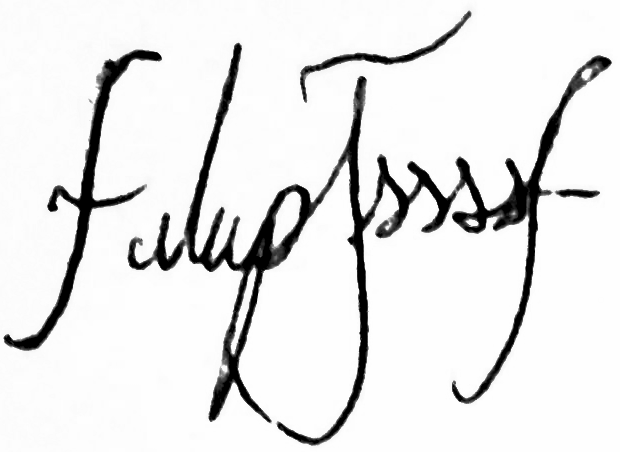
\includegraphics[width=120px,height=40px]{tex_open/support/corrected}\end{flushright} % signature
\fi

~\vfill
\begin{center}
	\begin{minipage}[c]{0.25\linewidth}
		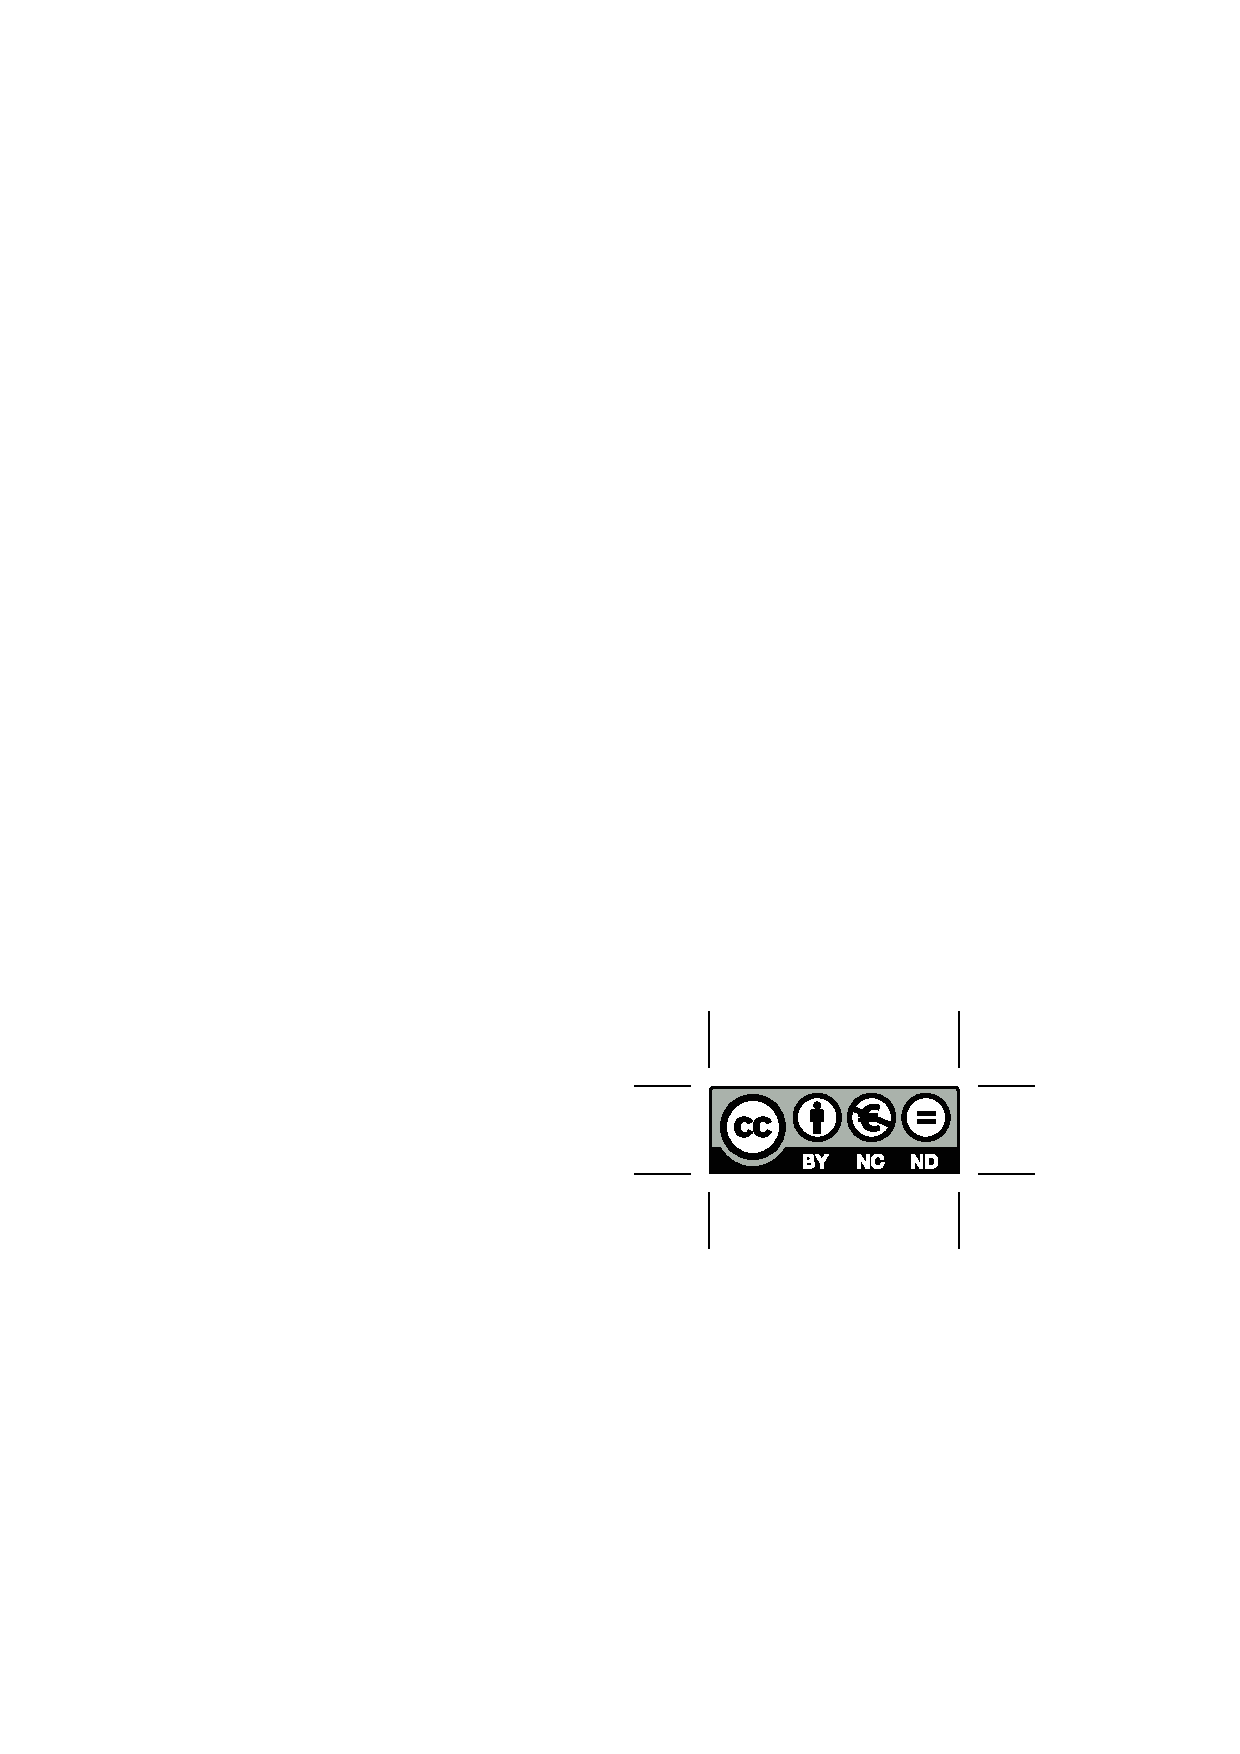
\includegraphics[height=35px]{by-nc-nd-eu}
	\end{minipage}\hfill
\end{center}

Cette \oe{}uvre est mise à disposition selon les termes de la \href{https://creativecommons.org/licenses/by-nc-nd/4.0/deed.fr}{Licence Creative Commons Attribution - Pas d’Utilisation Commerciale - Pas de Modification 4.0 International}. % consultez les conditions de la licence cc by-nc-nd, vous pouvez appliquer une licence moins restrictive, cc by-nc-sa par exemple
				%% affidavit et licence
	\newpage
\chapter*{Liste de publications et participation aux conférences}
\addcontentsline{toc}{chapter}{Liste de publications et participation aux conférences}
\subsection*{Liste des publications réalisées dans le cadre du projet de thèse:}
\begin{enumerate}
    \item Opti-CAM: Optimizing saliency maps for interpretability. (Pattern Recognition, under revision)
    \item CA-Stream: Attention-based pooling for interpretable image recognition. (-)
    \item A Learning Paradogm for Interpretable Gradients. (VISAPP 2024)
    \item The concept of Zero Information in Explainable AI
\end{enumerate}


\subsection*{Participation aux conférences et écoles d’été au cours de la période de thèse:}
\begin{enumerate}
\item ELLIS Summer School on Large-Scale AI for Research and Industry. Modène, Italie.
\end{enumerate}
			%% liste de publications et participation aux conférences
	%--------------------------------------------------------------------------------------------------
\chapter*{Résumé}
\addcontentsline{toc}{chapter}{Résumé}
Les applications de vision par ordinateur utilisant les technologies de l'intelligence artificielle 
ont connu une évolution remarquable au cours de la dernière décennie. Les développements actuels en 
vision par ordinateur sont le résultat direct d'une meilleure utilisation du matériel, permettant 
la construction de modèles capables d'effectuer des tâches plus complexes au fil du temps. En ce 
qui concerne la reconnaissance d'images en particulier, les réseaux neuronaux convolutionnels et 
les transformateurs sont désormais capables d'identifier les images et leurs éléments, ainsi que 
d'attribuer une valeur sémantique à ces derniers, même dans des conditions difficiles.\\

\noindent Avec la diffusion des technologies de l' apprentissage profond au sein de la société, 
une nouvelle exigence a émergé pour ces méthodologies. Puisqu 'elles interagissent désormais et 
affectent directement les vies humaines, il est impératif de comprendre leur fonctionnement et de 
fournir des explications. Pour répondre à ces questions, un nouveau domaine de recherche a vu le 
jour: l 'interprétabilité et l 'IA explicable.\\

\noindent Dans cette thèse, notre objectif est de comprendre et de développer des modèles 
d'interprétabilité pour les modèles de reconnaissance d'images de pointe. Nous présentons et 
expliquons brièvement certains des modèles de reconnaissance d'images les plus performants et 
pertinents pour les Réseaux de Neurones Convolutifs et les Transformers. Ensuite, nous examinons 
les approches actuelles en matière d' interpr\'etabilit\'e conçues pour fournir des explications, 
ainsi que leurs protocoles d' évaluation. Nous faisons des observations sur ces méthodes et 
protocoles d'évaluation, mettant en évidence les difficultés rencontrées et suggérant des idées 
pour surmonter leurs limitations.\\

\paragraph{Opti-CAM} Notre première contribution, s' appuie sur le raisonnement des Cartes d' 
Activation de Classe. En particulier, cette proposition optimise le coefficient de pondération 
requis pour calculer une carte de saillance, générant une représentation qui maximise la 
probabilité spécifique à la classe. Cette carte de saillance offre les meilleurs résultats selon 
les mesures d'interprétabilité, et met en évidence que le contexte est pertinent pour décrire une 
prédiction. De plus, une nouvelle métrique pour compléter l'évaluation de l'interprétabilité est 
dévoilée, remédiant aux lacunes de cette procédure.\\

\paragraph{Cross Attention Stream} Notre deuxième contribution, est un ajout aux modèles actuels de 
reconnaissance d'images, améliorant les mesures d'interprétabilité. Inspiré par des modèles 
novateurs performants tels que les Transformers, nous construisons un flux qui calcule l'interaction 
d'une représentation de classe abstraite avec les caractéristiques profondes des réseaux neuronaux 
convolutionnels. Cette représentation est finalement utilisée pour effectuer la classification. 
Notre flux affiche des améliorations lors de l'évaluation quantitative, tout en préservant les 
performances de reconnaissance à travers différents modèles.\\

\paragraph{Gradient Denoise} Enfin, notre dernière contribution présente un nouveau paradigme d' 
entraînement pour les réseaux neuronaux profonds. De plus, ce paradigme débruite les informations 
de gradient des modèles profonds dans l'espace d'entrée. La représentation de rétropropagation 
guidée de l'image d'entrée est utilisée pour régulariser les modèles lors de leur phase d' 
entraînement. En conséquence, nos modèles entraînés affichent des améliorations pour l' 
évaluation interprétable. Nous appliquons notre paradigme à de petites architectures dans un cadre 
contraint, ouvrant la voie au développement futur dans des ensembles de données à grande échelle, 
ainsi qu'avec des modèles plus complexes.\\

\vspace{0.5cm}
%Keywords: deep learning, image processing, attributions, interpretability
Mots clés: Apprentissage Profond, reconaissance d'image, interpretabilité, explicabilité.
					%% résumé
	%--------------------------------------------------------------------------------------------------
\chapter*{Abstract}
\addcontentsline{toc}{chapter}{Abstract}
Computer Vision applications using Artificial Intelligence technologies have undergone a remarkable 
evolution in the past decade. Current developments in Computer Vision are a direct result of a 
better utilization of hardware, enabling the construction of models capable of performing more 
complex tasks over time. On image recognition in particular, convolutional neural networks and 
transformers are now able to identify images and their elements, as well as assign semantic value 
to them, even in challenging conditions. These models have completely changed the landscape of deep 
learning and image recognition, permeating deep into society with the automatization of many daily 
tasks. Thus, it is no longer a question of \emph{can a model perform 
this task?}, but more a question of \emph{how does this model perform this task?}. To address these 
questions a new research field has emerged: interpretability and explainable AI.\\
\\
%Moreover, progress in this field has paved the way for further developments in complementary fields 
%of Computer Vision: models developed for image recognition are modified to conduct image 
%segmentation and reconstruction.\\

%\noindent The Deep Learning revolution occurred in two stages: first with the reemergence and 
%popularization of convolutional neural networks, and in second place with the 
%introduction of attention based architectures. On one hand, convolutional neural networks were 
%initially hard to train given their complexity and data volume requirements. 
%Still, early proposals showed promise, such as LeNet with the automatic recognition of handwritten 
%digits in the US postal service in the early 1990s. 
%However, in the early years of the last decade these issues were solved with the widespread of 
%large scale visual recognition datasets, as well as with the effective use of Graphics Processing 
%Units for computation. On the other hand, close to the end of this time period a new style of model 
%emerged: the Transformer architecture. This architecture creates an abstract representation of 
%lasses that interacts with every element of an encoding, generating a representation that learns a 
%class representation. Additionally, Transformers can process larger volumes of data, 
%allowing them to be robust to bias and generalize better.\\

%\noindent Convolutional Neural Networks and Transformers 
\noindent In this thesis, our goal is to understand and further develop interpretability models for 
state-of-the-art image recognition models. We introduce and briefly explain some of the most 
relevant high performance image recognition models for both Convolutional Neural Networks 
and Transformers. Then, current interpretability approaches designed to provide 
explanations, as well as their evaluation protocols. We make observations upon 
these methods and evaluation protocols, highlighting difficulties upon them and suggesting ideas 
to address their limitations.\\

\noindent In particular, a novel attribution method is proposed, ensuring that the highlighted 
regions in an image maximize a given class probability. From this method we observe that the 
most important information correlating to a class prediction, is not only found in the object of 
interest. Instead, context conveys salient information too: it is usually spread all over the image. 
Additionally, an addition to existing architectures is introduced, this method enhances predictive 
confidence, boosting interpretability properties of high performing image recognition models. Lastly, we 
propose a learning paradigm, that denoises gradients on the image space, enhancing 
interpretability properties. This final proposition demonstrates improvements on interpretability 
metrics for small datasets and models, while displaying promise for its scaling on to larger 
datasets and architectures.\\

\vspace{0.5cm}
Keywords: Deep Learning, image recognition, interpretability, explainability.

				%% abstract
	\chapter*{Remerciements}
\addcontentsline{toc}{chapter}{Remerciements}
Le modèle de thèse AMU n'existerait pas sans la contribution des doctorants. Nous souhaitons remercier tout particulièrement \href{http://www.theses.fr/2011AIX20720}{Mickaël Bojados}, \href{http://www.theses.fr/2011AIX22111}{Flora Cordoleani} et \href{http://www.theses.fr/2014AIXM4013}{Florian Caullery} pour leur aide précieuse et la qualité de leurs fichiers sources LaTeX. La mise à jour effectuée en 2018 doit beaucoup à l'excellent travail de \href{http://theses.fr/2014ENMP0038}{Dorian Depriester}.

\lipsum[1-2]\index{Nam dui ligula}
				%% remerciements

    \microtypesetup{protrusion=false}	%% désactive la protrusion (TOC LOFT GLS)
	\tableofcontents					%% TOC
	\listoffigures						%% LOF
	\listoftables						%% LOT
	\printglossary[						%% acronymes
		type=\acronymtype,
		title={Liste des acronymes},
		toctitle={Liste des acronymes}
		]
	\printglossary[						%% glossaire
		title={Glossaire},
		toctitle={Glossaire}
		]
	\printglossary[						%% nomenclature
		type=notation,
		title={Nomenclature},
		toctitle={Nomenclature}
		]
    \microtypesetup{protrusion=true}	%% rétabli la protrusion

	\ohead{\leftmark\Ifstr{\rightmark}{\leftmark}{}{ -- \rightmark}}	%% place le chapître et la partie en en-tête

    %--------------------------------------------------------------------------------------------------
\addchap{Introduction}
%\addcontentsline{toc}{chapter}{Introduction}
\noindent Amongst the sensory information that the brain processes, visual stimuli accounts 
for 90\% of data analyzed \autocite{potter2014detecting}, while consuming a great amount of energy 
in human metabolism (\cite{phelps1981metabolic}). It is argued that a big influence on the 
brain evolution was as a result of improving the capacity to process this kind of data and the 
ensuing  pattern recognition (\cite{mattson2014superior}). 
Currently, these shapes and forms have evolved too: it is no longer common for a human in most 
metropolitan areas, the need to scan the environment for faces that could reveal a potential 
predator; for a change, the patterns that we now seek to unravel also contain products of our own 
imagination: digits and characters, geometrical shapes.\\

\paragraph{Visual Recognition} Understanding the processes behind visual recognition has been a 
prominent research question throughout human history. From the preliminary questionings by greek  
philosphers (\cite{finger2001origins}) to physics based studies like those by Newton and Locke 
(\cite{swenson2010optics}), and more recently with theories like \textit{Unconscious Inference} 
(\cite{gullstrand1909hemholtz}) and \textit{Gestalt} (\cite{wagemans2012century}), many proposals 
to understand and describe this process have been brought forth. Moreover, vision recogniton is not 
only studied in fields like physics, medicine and psychology; 
with the advent of computer science, computational approaches and theories started emerging 
regarding this domain. One such study that proved seminal in this domain is that carried out by 
David Marr (\cite{poggio1981marr}, \cite{marr2010vision}). Most notably, Marr addressed vision on 
three levels: comptational, algorithmic and implementation. In particular, upon the computational 
level, Marr pondered around issues that the visual system answers and their explanation; this 
ultimately led to the formulation of fundamental tasks within computer vision such as object 
recognition and reconstruction. Over the past decade great advancements were made on computer 
vision. In particular with the optimization and popularization of \gls{gpu}, models requiring 
a strong computational power became accesible for researchers. To be specific, the framework 
developed by Yann LeCun (\cite{lecun1998gradient}) got revitalized in 2012 with the introduction of 
AlexNet (\cite{krizhevsky2012imagenet}) where proper leverage of these machines outclassed that of 
more traditional machine learning models, Chapter \ref{ch:rel} discusses this in more depth. 
In this short span of time, several groundbreaking architectures have been proposed, in 
particular the ResNet family (\cite{he2016deep}) has remained relevant given its properties
(\cite{wightman2021resnet}); furthermore, with the introduction of the transformer architecture 
(\cite{vaswani2017attention}) this field of research recieved a new impulse and more powerful 
models based upon its functional unit are being brought forth.\\

\noindent It is not only with the increase of computational power that computer vision has improved over time. 
With the developement, popularization and spread of the internet; large collections of data have been 
formed. These aggregations can be extremely specific for a given end, or 
quite general representing the common interests of its users. Over time, these compilations have 
continued to grow both in volume and variety; still, several curated collections are introduced by 
researchers to experiment and control the development of models such as MNIST (\cite{lecun1998gradient}),
BSDS (\cite{MartinFTM01}), Pascal VOC (\cite{pascal-voc-2012}) and most notably, 
ImageNet (\cite{ILSVRC15}) and MS-COCO (\cite{lin2014microsoft}). Additionally, data collection is
an ongoing and a never ending process; as such, the idea of a dataset containing all types of 
information is no longer deemded a dream but a reality that might come true aided by Big Data in 
the foreseeable future \autocite{chen2014big}.\\

\noindent Taking into consideration the aforementioned  increase on  both compute power and data 
availability, deep learning based models have been steadily adopted and assimiliated within society; 
nowadays its no longer so much a question \textit{whether can a model achieve a given task}, but 
rather a question on \textit{how can this given model perform this task}. Providing an answer to 
this question is paramount as human lives are now being directly affected by such kind of models. 
The main issue behind understanding deep models, lies within the size and complexity of deep 
architecttures, where providing interpretable explanations has lead to the surge of a novel field 
of research (\cite{guidotti2018survey}, \cite{bodria2021benchmarking}).

\paragraph{Interpretability}
To begin discussing about interpretability, one must ponder around its definition. 
Over the last decade, many authors have attempted to address to this question. One 
of the most notable discussions can be found within \emph{The Mythos of Model Interpretability} 
(\cite{mythos_interp}). In this work, Lipton argues that for a model to be interpretable it must 
display two properties, \emph{Transparency} and \emph{Post-Hoc Interpretability}. In one hand, 
\textit{Transparency} answers questions regarding the model structure, training and inference 
processes; while on another hand, \textit{Post-Hoc Interpretability} relates to the explanations 
and information that can be drawn of the model itself.

\noindent Considering these properties, we observe that as machine learning models grew in 
complexity; their transparent properties vanished proportionaly to their size. It can be argued 
that traditional models offer themselves to  transparency due to their straightforward formulation 
and inherent properties. Conversely, in terms of post-hoc interpretations, methods like decision 
trees \cite{breiman2017classification} can be pruned to study their performance by removing 
branches (\cite{lakkaraju2016interpretable},\cite{mothilal2020explaining}). 
On another hand, established techniques such as Principal Component Analysis \gls{pca} 
(\cite{wold1987principal}), can be used to gain insight within data leading to a prediction.\\

\noindent When studying deep models, we find that it is after their size and complexity that their 
interpretable propierties get hindered. Common Convolutional Neural Networks \glspl{cnn} 
rely convolution as their corner stone, coupled with non-linear operations such as 
ReLU (\cite{fukushima1975cognitron}), Sigmoid, and Softmax (\cite{hopfield1985neural}) among others.
This aggregation of convolutions on one hand enables these models to process large quantities of 
data, and to a certain extent generalize; however, it also results in an extensive parameter count,
often reaching of millions, and most recently, even billions (\cite{openai_compute}). The 
computational load required for inference, typically measured in \gls{gflops} further compounds 
complexity.\\

\noindent Among the properties proposed by Lipton, we observe that offering model transparency is a 
rather challenging task. While understanding the behaviour of convolutions and 
self-attention might seem straightforward, it is their aggregation and subsequent flow of information what 
makes this process intricate. Moreover, transparency encompases aspects related to both
inference and training. In this regard, while deep learning research is often seen as an open field;
complete transparency is often disregarded as some authors frequently omit key details in their 
descriptions and methodologies. 

In contrast to transparency, providing post-hoc interpretations from deep models is a 
thriving field, where many of the challenges found within transparency are no longer found.
Within this field, various approaches have been proposed to achieve post-hoc interpretability,
including input masking (\cite{petsiuk2018rise}), attribution generation (\cite{NIPS2017_7062}, 
\cite{zhou2016learning}) and model perturbations 
(\cite{fong2017interpretable}, \cite{fong2019understanding}). Furthermore, the development of 
evaluation methodologies for these approaches has continued in tandem with them 
(\cite{choe2020evaluating}, \cite{chattopadhay2018grad}). Chapter \ref{ch:rel} delves deeper into 
these works. 

\paragraph{Dissertation Outline}
%\addcontentsline{toc}{section}{Dissertation Outline}
\noindent This dissertation is organized in the following manner: In Chapter \ref{ch:rel} we 
introduce a background for image recognition models (Section \ref{rel:sec_imrecon}) and the ensuing 
approaches developed to study the interpretability on them (Section \ref{rel:sec_int}). 
Additionally, we introduce evaluation procedures for these approaches which will be further used to 
evaluate ourproposals.\\

\noindent In Chapter \ref{ch:opticam}, we propose Opti-CAM as a methodology that generates 
optimized saliency maps highlighting the relevant regions on an image towards image classification. 
In Section \ref{sec:av_gain} we extend existing evaluation metrics with a novel measurement for 
model coinfidence. 
In Sections \ref{sec:oc_qual} and \ref{sec:oc_quant} we evaluate the effect of these contributions 
towards interpretability assessment.\\

\noindent Chapter \ref{ch:castream} introduces the Cross Attention Stream, an approach that boosts existing 
architectures interpretable properties. We ste up the modulus of this approach in 
Section \ref{sec:ca_defn} alongside its deployment on Section \ref{sec:ca_design}. 
In Sections \ref{sec:ca_qual} and \ref{sec:ca_quant} we demonstrate the benefits of using this
proposal.\\

\noindent Chapter \ref{ch:grad} characterizes a gradient denoising approach with a gradient denoising 
methodology as an approach to enhance the trainining procedure of current models while improving 
interpretability properties. In Section \ref{sec:grad_defn}, we define the gradient denoising 
protocol alongside the regularization proposals to do so.
Sections \ref{sec:grad_qual} and \ref{sec:grad_quant} illustrate the effects of this paradigmn
in the trained models and its effects on interpretability.\\

\noindent Chapter \ref{ch:zip} raises the Zero-Information algorithm and its usage as a substitute
for mask-dependent evaluation proposals. Section \ref{sec:zip_algo} develops this 
method. Section \ref{sec:zip_insdel} demonstrates its incorporation of this 
algorithm onto evaluation protocols. Section \ref{sec:zip_qual} displays
the effect of this approach when applied to mask patches on images. Section 
\ref{sec:zip_benchmark} displays the results of benchmarking these protocols 
with this approach. \\
    
\noindent Finally, we draw conclusions on our work and detail future research perspectives.
    \chapter{Related Work}
\addcontentsline{toc}{chapter}{Related Work}

\section{Image Recognition Models}

\subsection{Convolutional Neural Networks}

\subsection{Attention-Based Architectures}


\section{Interpretability}

\subsection{Transparency}

\subsection{Post-Hoc Interpretability}



%\lipsum[1-2]

	\chapter{Opti-CAM: Optimizing saliency maps for interpretability}
\chaptertoc{}
%--------------------------------------------------------------------------------------------------
\label{ch:opticam}
% Introduction, to move to a more verbatum approach
\section{Introduction}
\label{sec:oc_intro}
\noindent Within existing attribution approaches for interpretable saliency map generation, the CAM 
\autocite{zhou2016learning} based family of methods takes special interest given its reliance of
existing  information and properties of a given model to generate explanations. In particular, we 
note that following \autoref{eq:sal}, modifying computation of the weighting coefficient 
$w_k^c$ results in a different attribution being generated. Moreover, this computation can be altered,
 for instance by relying on information found while performing the backward pass 
 (\cite{selvaraju2017grad}, \cite{chattopadhay2018grad}, \cite{axiombased}, 
 \cite{smilkov2017smoothgrad}) and the forward pass \autocite{wang2020score} of the model during 
 inference. Nevertheless, we observe that among existing weighting coefficient computation 
 proposals, none has been directed at maximizing the predicted probability of the generated 
 saliency maps.

Complementary to CAM methods, we observe that within attribution methods based on extremal 
perturbations \autocite{fong2019understanding} or IBA \autocite{schulz2020restricting}, 
their class scores are optimized via gradient descent. In this regard, it can 
be stated that these masks then become variables within input-feature space, and the aforementioned 
scores then become a function of said masking. However it is important to point that optimizing 
these masks ultimately becomes an expensive process, as several constraints are needed 
to be taken into consideration to further control the masking area.

Drawing inspiration from the aforementioned observations, we set ourselves to design \emph{Opti-
CAM}, an attribution method that generates saliency maps with enhanced interpretability. In 
particular, we hypothesize that the weighting coefficient $w_k^c$ can be optimized to attain this 
task; moreover, we also suggest that should the predicted probability of the attribution map is 
optimized, we can gain insight within the regions of the image that appear to be the most important 
for the classifier. We define our approach in \autoref{sec:oc_def}\\

\noindent In addition to the proposal of an attribution method in this chapter, we aim towards the 
design of a complementary interpretability evaluation metric of saliency maps. In particular, 
based on the remarks found in Fake-CAM \autocite{poppi2021revisiting}; where it is noted that 
existing metrics such as \gls{ad} (\ref{eq:ad}) and \gls{ai} (\ref{eq:ai}) can be manipulated. As a 
result of this, we argue that a complementary criterion is missing regarding \textit{Objective 
Evaluation for Object Recognition}. In \autoref{sec:av_gain} we define this novel measurement 
under the name \gls{ag}. To support our approach, we demonstrate our generated saliency maps in 
\autoref{sec:oc_qual} and we evaluate them in \autoref{sec:oc_quant} and \autoref{sec:oc_loc}.

\noindent To sum up, with the observations previously mentioned, in this chapter we propose a CAM 
variant that generates saliency maps by optimizing the weighting coefficient $w_k^c$, while also 
introducing a novel metric to complement the existing evaluation of attribution methods.\\

\section{Preliminaries}
\label{sec:oc_prelim}

\paragraph{Notation}
\label{sec:oc_notation}

Consider a classifier network $f: \cX \to \real^C$ that maps an input image $\mathbf{u} \in \cX$ to a 
logit vector $\vy = f(\mathbf{u}) \in \real^C$, where $\cX$ is the image space and $C$ is the number 
of classes. We denote by $y_c = f(\mathbf{u})_c$ the predicted logit and by $p_c = \softmax(\vy)_c 
\defn e^{y_c} / \sum_j e^{y_j}$ the predicted probability for class $c$. For layer $\ell$ 
with $K_\ell$ channels, we denote by $A^k_\ell = f^k_\ell(\mathbf{u}) \in \real^{h_\ell \times w_\ell}$ 
the feature map for channel $k \in \{1,\dots,K_\ell\}$, with spatial resolution $h_\ell \times 
w_\ell$. Because of $\relu$ non-linearities, we assume that feature maps are non-negative. 
Similarly, we denote by $S_\ell \in \real^{h_\ell \times w_\ell}$ a 2D saliency map.

%--------------------------------------------------------------------------------------------------

\paragraph{Background: CAM-based saliency maps}
\label{sec:oc_back}

Given a layer $\ell$ and a class of interest $c$, we consider saliency maps given by the general 
formula
\begin{equation}
	S^c_\ell(\mathbf{u}) \defn h \left( \sum_k w^c_k A^k_\ell \right),
\label{eq:sal}
\end{equation}
where $w^c_k$ are weights defining a linear combination over channels and $h$ is an activation 
function. CAM \parencite{zhou2016learning} is defined for the last layer $L$ only with $h$ being the 
identity mapping and $w^c_k$ being the classifier weight connecting the $k$-th channel with 
class $c$. Grad-CAM \parencite{selvaraju2017grad} is defined for any layer $\ell$ with $h = \relu$ and 
weights
\begin{equation}
	w^c_k \defn \gap \left( \pder{y_c}{A^k_\ell} \right),
\label{eq:gcam}
\end{equation}
where $\gap$ is global average pooling.
% and $\softmax(\vy)_c = e^{y_c} / \sum_j e^{y_j}$ is the predicted probability of class $c$.
The motivation for $\relu$ is that we are only interested in features that have a positive effect 
on the class of interest, \ie pixels whose intensity should be increased in order to increase $y_c$.

Score-CAM \parencite{wang2020score} is also defined for any layer $\ell$ with $h = \relu$ and weights 
$w^c_k \defn \softmax(\mathbf{u}^c)_k$.  Softmax normalization considers positive channel contributions 
only and attends to few feature maps.
%that \alert{produce less highlighted areas in the saliency map}. \iavr{Last part unclear.}
Here, vector $\mathbf{u}^c \in \real^{K_\ell}$ measures the increase in confidence for class $c$ that 
compares a known baseline image $\mathbf{u}_b$ with the input image $\mathbf{u}$ masked according to feature 
map $A^k_\ell$, for all channels $k$:

\begin{equation}
	u^c_k \defn f(\mathbf{u} \odot n(\operatorname{up}( A^k_\ell )))_c - f(\mathbf{u}_b)_c,
\label{eq:s-cam}
\end{equation}

where $\odot$ is the Hadamard product. For this to work, the feature map $A^k_\ell$ is adapted
 to $\mathbf{u}$ first$:\operatorname{up}$ denotes upsampling to the spatial resolution of $\mathbf{u}$ and

\begin{equation}
	n(A) \defn \frac{A - \min A}{\max A - \min A}
\label{eq:norm}
\end{equation}

is a normalization of matrix $A$ into $[0,1]$. While Score-CAM does not need gradients, 
it requires as many forward passes through the network as the number of channels in the chosen layer,
 which is computationally expensive.

%--------------------------------------------------------------------------------------------------

\paragraph{Motivation}
\label{sec:motiv}

\iavr{Score-CAM considers each feature map as a mask in isolation. How about linear combinations?} 
Given a vector $\vw \in \real^{K_\ell}$ with $w_k$ its $k$-th element, let
\begin{equation}
	F(\vw) \defn f \left( \mathbf{u} \odot n \left( \operatorname{up} \left(
		\displaystyle\sum_k w_k A^k_\ell
	\right) \right) \right)_c.
\label{eq:s-obj}
\end{equation}
\ronan{If we assume that $\mathbf{u}_b = \vzero$ in~\eq{s-cam} and define $n(\vzero) \defn \vzero$ 
in~\eq{norm}, then we can rewrite the right-hand side of~\eq{s-cam} as
\begin{equation}
	\frac{F(\vw_0 + \delta \ve_k) - F(\vw_0)}{\delta},
\label{eq:s-cam2}
\end{equation}
where $\vw_0 = \vzero$, $\delta = 1$ and $\ve_k$ is the $k$-th standard basis vector of 
$\real^{K_\ell}$. This resembles the numerical approximation of the derivative $\pder{F}{w_k}(\vw_0)$,
 except that $\delta$ is not small as usual. One could compute derivatives efficiently by 
 standard backpropagation instead. It is then possible to iteratively optimize $F$ with respect
  to $\vw$, starting at any $\vw_0$.}

\iavr{As an alternative, consider masking-based methods relying on optimization in the input space, 
like \emph{meaningful perturbations} (MP) \parencite{fong2017interpretable} or 
\emph{extremal perturbations} \parencite{fong2019understanding}. In general, optimization takes the form
\begin{equation}
	S^c(\mathbf{u}) \defn \arg\max_{\vm \in \cM} f(\mathbf{u} \odot n(\operatorname{up}(\vm)))_c + \lambda R(\vm).
\label{eq:mask}
\end{equation}
Here, a mask $\vm$ is directly optimized and does not rely on feature maps, hence the saliency 
map $S^x(\mathbf{u})$ is not connected to any layer $\ell$. The mask is at the same or lower resolution 
than the input image. In the latter case, upsampling is still necessary.

In this approach, one indeed computes derivatives by backpropagation and indeed iteratively 
optimizes $\vm$. However, because $\vm$ is high-dimensional, there are constraints expressed by 
$\vm \in \cM$, \eg $\vm$ has a certain norm, and regularizers like $R(\vm)$, \eg $\vm$ is smooth in a 
certain way. This makes optimization harder or more expensive and introduces more hyperparameters 
like $\lambda$. One could simply constrain $\vm$ to lie in the linear span of $\{A_\ell^k\}_{k=1}
^{K_\ell}$ instead, like all CAM-based methods.}
\section{Opti-CAM}
As motivated by \textbf{motif}, we obtain a saliency map as a convex combination of feature maps
 by optimizing a given objective function with respect to the weights.
In particular, following \autocite{wang2020score}, we use channel weights $w_k \defn \softmax(
	\mathbf{u})_k$, where $\mathbf{u} \in \real^{K_\ell}$ is a variable.
We then consider saliency map $S_\ell$ in layer $\ell$ as a function of both the input image $\vx$ 
and variable $\mathbf{u}$:

\begin{equation}
    S_\ell(\vx; \mathbf{u}) \defn \sum_k \softmax(\mathbf{u})_k A^k_\ell.
\label{eq:v-sal}
\end{equation}
Comparing with \eq{sal}, $h$ is the identity mapping, because feature maps are non-negative and
 weights are positive.

%--------------------------------------------------------------------------------------------------

\subsection{Optimization}
Now, given a layer $\ell$ and a class of interest $c$, we find the vector $\mathbf{u}^*$ that
 maximizes the classifier confidence for class $c$, when the input image $\vx$ is masked according 
 to saliency map $S_\ell(\vx; \mathbf{u}^*)$:
\begin{equation}
	\mathbf{u}^* \defn \arg\max_{\mathbf{u}} F^c_\ell(\vx; \mathbf{u}),
\label{eq:opt}
\end{equation}

where we define the objective function
\begin{equation}
	F^c_\ell(\vx; \mathbf{u}) \defn g_c(f(\vx \odot n(\up(S_\ell(\vx; \mathbf{u}))))).
\label{eq:obj}
\end{equation}
Here, the saliency map $S_\ell(\vx; \mathbf{u})$ is adapted to $\vx$ exactly as in~\eq{s-cam} in 
terms of resolution and normalization. For \emph{normalization function} $n$, the default is
 \eq{norm}. 
The \emph{selector function} $g_c$ operates on the logit vector $\vy$; the default is to select the
 logit of class $c$, \ie $g_c(\vy) \defn y_c$. %Other choices, including the definition of
 %$F^c_\ell$ itself, are investigated in \autoref{sec:ablation} \redred{and in the supplementary material.}

%--------------------------------------------------------------------------------------------------
\begin{figure}[t]
    \centering
    % \fig[.8]{method/OptiCAM-1.png}
    %------------------------------------------------------------------------------
    \resizebox{\textwidth}{!}{%
    \begin{tikzpicture}[
        scale=.12,
        font={\small},
        node distance=.2,
        label distance=2pt,
        net/.style={draw,trapezium,trapezium angle=75,inner sep=3pt},
        enc/.style={net,shape border rotate=270},
        txt/.style={inner sep=3pt},
        frame/.style={draw,minimum size=1cm},
        feat/.style={frame},
        sq/.style={minimum size=.15cm},
        elem/.style={draw,sq},
        vec/.style={draw,minimum width=.8cm,minimum height=.15cm},
        var/.style={blue!60},
        B/.style={fill=blue!20},
        R/.style={fill=red!20},
        G/.style={fill=green!20},
        Y/.style={fill=yellow!40},
        P/.style={fill=black!20},
    ]
    \matrix[
        tight,row sep=0,column sep=14,
        cells={scale=.3,},
    ] {
        \&\&\&\&\&\&\&
    % 	\node[var,op] (error) {$-$}; \&
        \node[txt] (loss) {objective \\ $F^c_\ell(\vx; \mathbf{u})$}; \\
        \node[label=90:{input image $\vx$}] (in) {\figah[1.5cm]{opticam/images/idea/input}}; \&
        \node[enc] (net) {network \\ $f$}; \&
        \foreach \s/\c in {-2/B,-1/R,0/G,1/Y,2/P}
            {\node[feat,\c] (feat\s) at ($.4*(\s,-\s)$) {};}
        \node        at (feat2) {\figah[1cm]{opticam/images/idea/27_fea0}};
        \node[frame] at (feat2) {};
        \coordinate[label=90:{feature \\ maps $A^k_\ell$}]
                    (feat-north) at (feat-2.north -| feat0.north);
        \coordinate (feat-west)  at (feat-2.west  |- feat0.west);
        \coordinate (feat-east)  at (feat2.east   |- feat0.east);
        \&
        \node[var,op] (cam) {$\times$};
        \foreach \s/\c in {-2/B,-1/R,0/G,1/Y,2/P}
            {\node[elem,\c] (elem\s) at ($.6*(\s,-6)$) {};}
        \node[sq,label=-90:{weights $\mathbf{u}$}] (weight) at (elem0) {};
        \&
        \node[var,label=90:{saliency map \\ $S_\ell(\vx; \mathbf{u})$}] (sal) {\figah[1.5cm]{opticam/images/idea/saliency}}; \&
        \node[var,op] (mask) {$\odot$}; \&
        \node[label=90:{masked image}] (masked) {\figah[1.5cm]{opticam/images/idea/masked}}; \&
        \node[enc] (net2) {network \\ $f$}; \\[8]
        \&\&\&
        \coordinate (mid); \\
    };
    
    \draw[->]
        (in) edge (net)
        (net) edge (feat-west)
        (feat-east) edge (cam)
        (net2) edge node[pos=.5,right] {class \\ logits} (loss)
    % 	(net) |- node[pos=.3,left] {class \\ logits} (error)
        ;
    
    \draw[var,->]
        (weight) edge (cam)
        (cam) edge (sal)
        (sal) edge (mask)
        (mask) edge (masked)
        (masked) edge (net2)
    % 	(net2) edge (error)
    % 	(error) edge (loss)
        (net2) edge (loss)
        ;
    
    \draw[->]
        (in) |- (mid)
        (mid) -| (mask)
        ;
    
    \end{tikzpicture}
    }
% \vspace{6pt}
\caption{Overview of Opti-CAM. We are given an input image $\vx$, a fixed network $f$, a target layer $\ell$ and a class of interest $c$. We extract the feature maps from layer $\ell$ and obtain a saliency map $S_\ell(\vx; \mathbf{u})$ by forming a convex combination of the feature maps ($\times$) with weights determined by a variable vector $\mathbf{u}$~\eq{v-sal}. After upsampling and normalizing, we element-wise multiply ($\odot$) the saliency map with the input image to form a ``masked'' version of the input, which is fed to $f$. The objective function $F^c_\ell(\vx; \mathbf{u})$ measures the logit of class $c$ for the masked image~\eq{obj}. We find the value of $\mathbf{u}^*$ that maximizes this logit by optimizing along the path highlighted in blue~\eq{opt}, as well as the corresponding optimal saliency map $S_\ell(\vx; \mathbf{u}^*)$~\eq{o-sal}.}
\label{fig:idea}
\vspace{-0.4cm}
\end{figure}
Putting everything together, we define
\begin{equation}
	S^c_\ell(\vx) \defn S_\ell(\vx; \mathbf{u}^*) = S_\ell(\vx; \arg\max_{\mathbf{u}} F^c_\ell(\vx;
	\mathbf{u})),
\label{eq:o-sal}
\end{equation}
where $S_\ell$ and $F^c_\ell$ are defined by~\eq{v-sal} and~\eq{obj} respectively. The objective 
function $F^c_\ell$ ~\eq{obj} depends on variable $\mathbf{u}$ through $S_\ell$~\eq{v-sal}, where
 the feature maps $A^k_\ell = f^k_\ell(\vx)$ are fixed. Then,~\eq{obj} involves masking and a
  forward pass  through the network $f$, which is also fixed.

Figure \ref{fig:idea} is an abstract illustration of our method, \iavr{called Opti-CAM}, without 
details like upsampling and normalization~\eq{obj}. Optimization takes place along the highlighted 
path from variable $\mathbf{u}$ to objective function $F^c_\ell$. The saliency map is real-valued 
and the entire objective function is differentiable in $\mathbf{u}$. We use Adam optimizer 
\autocite{kingma2014adam} to solve the optimization problem ~\eq{opt}.


%--------------------------------------------------------------------------------------------------

%\paragraph{Discussion}

%By maximizing~\eq{obj}, the saliency map focuses on the regions contributing to class $c$, while masked regions contribute less. This way, the influence of background in the average pooling process is reduced.

%The saliency map is expressed as a linear combination of feature maps~\eq{v-sal}, with normalized weights. Hence, the saliency map is discouraged from taking up the entire image, both by the $\softmax$ competition~\eq{v-sal} and by the fact that feature maps only respond to particular locations.

%\iavr{In case $g_c(\vy) \defn y_c$,~\eq{o-sal} takes the form of direct masking~\eq{mask} with $R(\vm) = \vzero$ and
%\begin{equation}
%	\cM \defn \{ S_\ell(\vx; \mathbf{u}) : \mathbf{u} \in \real^{K_\ell} \}.
%\label{eq:mask-m}
%\end{equation}
%This constraint makes ours a CAM-based method. It dispenses the need for regularizers, because we only optimize one vector over the feature dimensions\modify{ (up to 2,048 for ResNet50), which is small compared with the dimensions of input images (50k for ImageNet)}. In addition, it does not complicate the optimization process in any way. It is only a different parametrization.}
%--------------------------------------------------------------------------------------------------
\section{Average Gain}
\label{sec:av_gain}
Continuing on with observations of CAM-based Saliency maps, we recall the observation made for 
\emph{Fake-CAM} \cite{poppi2021revisiting}. In particular, we note that traditional 
interpretability measurements such as \gls{ad} and \gls{ai} can be deceiving; as perfect scores can 
be nearly achieved for \gls{ad} by masking all but one pixel in the Saliency Map. This is used to 
motivate the definition of a number of metrics that are orthogonal to the task at hand, \ie 
measuring the effect of masking to the classifier. By contrast, we address the problem by 
introducing a new metric to be paired with $\AD$ as a replacement of $\AI$: 
\emph{Average Gain}.\\

\noindent \emph{\glsfirst{ag}} quantifies how much predictive power, measured as class probability; 
is gained when we mask the image. We define this metric in the following manner, where higher is 
better:
\begin{equation}
	\AG(\%) \defn \frac{1}{N} \sum_{i=1}^N \frac{[o^c_i - p^c_i]_+}{1-p^c_i} \cdot 100.
\label{eq:ag}
\end{equation}
This definition is symmetric to the definition of average drop, in the sense that in absolute value,
the numerator in the sum of $\AD, \AG$ is the positive and negative part of $p^c_i - o^c_i$ 
respectively and the denominator is the maximum value that the numerator can get as a function of 
$o^c_i$, given that $0 < o^c_i < p^c_i$ and $p^c_i < o^c_i < 1$ respectively. The two metrics thus  
compete each other, in the sense that changing $o^c_i$ to improve one leaves the other unchanged or  
harms it. As we shall see, an extreme example is Fake-CAM, which yields near-perfect $\AD$ but 
fails completely on $\AG$.


%--------------------------------------------------------------------------------------------------
\section{Experiments}
\label{sec:oc_exp}
We evaluate Opti-CAM and compare it quantitatively and qualitatively against other state-of-the-art 
methods on a number of datasets and networks. We report classification metrics with execution times, 
and we provide visualizations, an ablation study and a study on the suitability of localization 
ground truth.
%A sanity check, additional classification results, localization metrics, more ablations, more 
%visualizations \redred{and code} are given in supplementary material}

\subsection{Implementation details}
\label{sec:oc_details}

All input images are resized to $224 \times 224 \times 3$. To optimize the saliency map with 
Opti-CAM~\eq{opt}, we use the Adam \autocite{kingma2014adam} optimizer with learning rate $0.1$ by 
default, setting the maximum number of iterations to $100$ and stopping early when the change in 
loss is less than $10^{-10}$. For VGG16, we generate the saliency map \eq{v-sal} from the feature 
maps of the last convolutional layer before max pooling by default, \ie convolutional layer 3 of 
block 5. For ResNet50, we choose the last convolutional layer by default, \ie convolutional layer 3 
of bottleneck 2 of block 4. For ViT and DeiT, we choose the last self-attention block by default, 
\ie layer normalization of self-attention block 12. 

\subsection{Datasets}
\label{sec:oc_data}

\paragraph{ImageNet}
We use the validation set of ImageNet ILSVRC 2012 (\cite{krizhevsky2012imagenet}, \cite{ILSVRC15}), 
containing $50,000$ images evenly distributed over the $1,000$ categories. For the ablation study 
and for timing, we sample $1,000$ images from this set. Concerning the localization experiments, 
bounding boxes from the localization task of ILSVRC
\footnote{\url{https://www.image-net.org/challenges/LSVRC/2012/index.php}} are used on the same 
validation set.

\paragraph{Medical data}

We use two medical image datasets, namely \emph{Chest X-ray} \autocite{kermany2018labeled} and 
\emph{Kvasir} \autocite{pogorelov2017kvasir}. 
%Complete qualitative and quantitative results are given 
%in the supplementary. Here we only provide visualizations.

%--------------------------------------------------------------------------------------------------

\paragraph{Networks}
\label{sec:oc_setup}

For all datasets, we use the pretrained ResNet50 \autocite{he2016deep} and VGG16 
\autocite{simonyan2015deep} networks with batch normalization \autocite{ioffe2015batch} from the 
Pytorch model zoo\footnote{\url{https://pytorch.org/vision/0.8/models.html}}. For ImageNet, we 
further use the pretrained ViT-B (16-224) \autocite{dosovitskiy2020image} and DeiT-B (16-224) 
\autocite{pmlr-v139-touvron21a} from Pytorch image models (timm)\footnote{\url{
    https://github.com/rwightman/pytorch-image-models}}.
% pre-trained on ImageNet-21k and fine-turned on ImageNet-1k~\autocite{ILSVRC15}.
%Regarding medical datasets, we fine-tune the networks as discussed in the supplementary material, 
%where we also provide the setting details.


%--------------------------------------------------------------------------------------------------

\subsection{Evaluation}
\label{sec:eval}

\paragraph{Metrics}
We use \emph{\gls{ad}} and \emph{\gls{ai}} \autocite{chattopadhay2018grad} metrics, as well 
as the proposed \emph{\gls{ag}}, to measure the effect on classification performance of masking 
the input image by a saliency map. In addition, we report \emph{\gls{ins}} and \emph{\gls{del}}  
\autocite{petsiuk2018rise} and highlight their limitations. Using classification metrics, we show 
the limitations of using the localization ground truth for the evaluation of attribution methods. 
In \autoref{sec:oc_wsol}, we provide a number of localization metrics from the 
\emph{weakly-supervised object localization} (WSOL) task of ILSVRC2014
\footnote{\url{https://www.image-net.org/challenges/LSVRC/2014/index\#}}.

\paragraph{Methods}

We compare against the following state-of-the-art methods: Grad-CAM \autocite{selvaraju2017grad}, 
Grad-CAM++\cite{chattopadhay2018grad}, Score-CAM \autocite{wang2020score}, Ablation-CAM 
\autocite{ramaswamy2020ablation}, XGrad-CAM \autocite{axiombased}, Layer-CAM 
\autocite{jiang2021layercam}, ExtremalPerturbation \autocite{fong2019understanding} 
and HiRes-CAM \autocite{draelos2020use}. Implementations are obtained from the PyTorch CAM 
library\footnote{\url{https://github.com/jacobgil/pytorch-grad-cam}} or 
TorchRay\footnote{\url{https://github.com/facebookresearch/TorchRay}}. For transformer models, 
we also compare against raw attention \autocite{dosovitskiy2020image}, 
rollout \autocite{abnar2020quantifying} and TIBAV \cite{chefer2021transformer}\footnote{\url{
https://github.com/hila-chefer/Transformer-Explainability}}.

\paragraph{Image normalization}

It is standard that images are normalized before feeding them to a network. By doing so however, 
we cannot reproduce the results published for the baseline methods; rather, all results are 
improved dramatically. We can obtain results similar to published ones by \emph{not} normalizing. 
We believe normalization is important, and we include it in all our experiments. 
%--------------------------------------------------------------------------------------------------
\section{Qualitative Evaluation}
\label{sec:oc_qual}
\begin{figure}[H]
    \newcommand{\sizeS}{.125}
    \newcommand{\sizeP}{.125}
    \newcommand{\hh}{.175\textwidth}
    \newcommand{\ww}{.200\textwidth}
    \setlength{\tabcolsep}{2pt}
    \centering
    \scriptsize
    %\setlength{\tabcolsep}{2pt}
    \begin{tabular}{cccccccc}
        & Input image &  Grad-CAM  & Grad-CAM++ & Score-CAM & Ablation-CAM & XGrad-CAM & Opti-CAM 
     \\
    
        \rotatebox{90}{~Grass Snake} &
        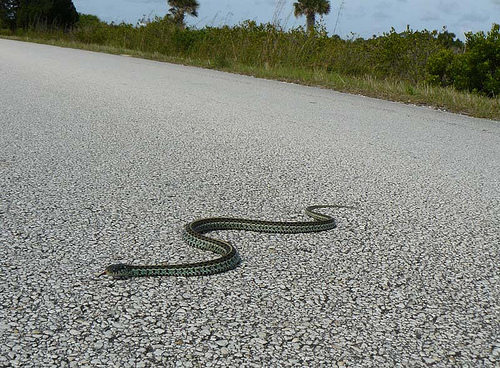
\includegraphics[trim={36mm 10mm 32mm 10mm},clip, width=\sizeP\textwidth]{fig/opticam/images/select/ILSVRC2012_val_00000006.JPEG}&
        \fig[\sizeS]{opticam/images/select/ILSVRC2012_val_00000006JPEG_vgg_GradCAM_vis.png} &
        \fig[\sizeS]{opticam/images/select/ILSVRC2012_val_00000006JPEG_vgg_GradCAMPlusPlus_vis.png} &
        \fig[\sizeS]{opticam/images/select/ILSVRC2012_val_00000006JPEG_vgg_ScoreCAM_vis.png} &
        \fig[\sizeS]{opticam/images/select/ILSVRC2012_val_00000006JPEG_vgg_AblationCAM_vis.png} &
        \fig[\sizeS]{opticam/images/select/ILSVRC2012_val_00000006JPEG_vgg_XGradCAM_vis.png} &
        \fig[\sizeS]{opticam/images/select/ILSVRC2012_val_00000006JPEG_vgg_versionP0_vis.png}  \\
    
        \rotatebox{90}{~Tricycle} &
        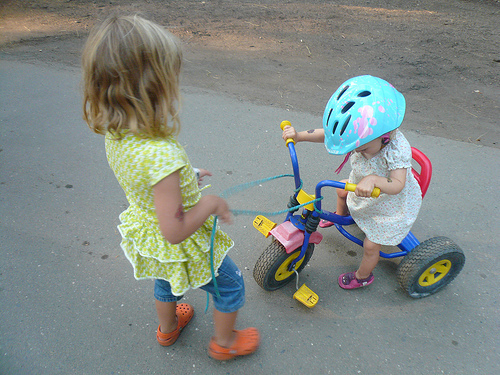
\includegraphics[trim={28mm 10mm 39mm 10mm},clip, width=\sizeP\textwidth]{fig/opticam/images/select/ILSVRC2012_val_00000069.JPEG}&
        \fig[\sizeS]{opticam/images/select/ILSVRC2012_val_00000069JPEG_vgg_GradCAM_vis.png} &
        \fig[\sizeS]{opticam/images/select/ILSVRC2012_val_00000069JPEG_vgg_GradCAMPlusPlus_vis.png} &
        \fig[\sizeS]{opticam/images/select/ILSVRC2012_val_00000069JPEG_vgg_ScoreCAM_vis.png} &
        \fig[\sizeS]{opticam/images/select/ILSVRC2012_val_00000069JPEG_vgg_AblationCAM_vis.png} &
        \fig[\sizeS]{opticam/images/select/ILSVRC2012_val_00000069JPEG_vgg_XGradCAM_vis.png} &
        \fig[\sizeS]{opticam/images/select/ILSVRC2012_val_00000069JPEG_vgg_versionP0_vis.png}  \\

        \rotatebox{90}{~Komondor} &
        \fig[\sizeS]{opticam/images/visual/ILSVRC2012_val_00001113.png}&
        \fig[\sizeS]{opticam/images/visual/Resnet50_GradCAM_ILSVRC2012_val_00001113.png} &
        \fig[\sizeS]{opticam/images/visual/Resnet50_GradCAMPlusPlus_ILSVRC2012_val_00001113.png} &
        \fig[\sizeS]{opticam/images/visual/Resnet50_ScoreCAM_ILSVRC2012_val_00001113.png} &
        \fig[\sizeS]{opticam/images/visual/Resnet50_AblationCAM_ILSVRC2012_val_00001113.png} &
        \fig[\sizeS]{opticam/images/visual/Resnet50_XGradCAM_ILSVRC2012_val_00001113.png} & 
        \fig[\sizeS]{opticam/images/visual/Resnet50_OptCAM_ILSVRC2012_val_00001113.png}  \\
            
        \rotatebox{90}{~Pneumonia} &
        \fig[\sizeS]{opticam/images/medical/chest_VGG16_GradCAM_1_img.png} &
        \fig[\sizeS]{opticam/images/medical/chest_VGG16_GradCAM_1_vis.png} &
        \fig[\sizeS]{opticam/images/medical/chest_VGG16_GradCAMPlusPlus_1_vis.png} &
        \fig[\sizeS]{opticam/images/medical/chest_VGG16_ScoreCAM_1_vis.png} &
        \fig[\sizeS]{opticam/images/medical/chest_VGG16_AblationCAM_1_vis.png} &
        \fig[\sizeS]{opticam/images/medical/chest_VGG16_XGradCAM_1_vis.png} &
        \fig[\sizeS]{opticam/images/medical/chest_VGG16_OptCAM_plain_1_vis.png}  \\
    
    
        \rotatebox{90}{~Pylorus} &
        \fig[\sizeS]{opticam/images/medical/kvasir_Resnet50_GradCAM_3_img.png} &
        \fig[\sizeS]{opticam/images/medical/kvasir_VGG16_GradCAM_3_vis.png} &
        \fig[\sizeS]{opticam/images/medical/kvasir_VGG16_GradCAMPlusPlus_3_vis.png} &
        \fig[\sizeS]{opticam/images/medical/kvasir_VGG16_ScoreCAM_3_vis.png} &
        \fig[\sizeS]{opticam/images/medical/kvasir_VGG16_AblationCAM_3_vis.png} &
        \fig[\sizeS]{opticam/images/medical/kvasir_VGG16_XGradCAM_3_vis.png} &
        \fig[\sizeS]{opticam/images/medical/kvasir_VGG16_OptCAM_plain_3_vis.png}  \\
    
    \end{tabular}
    \caption{\textbf{Saliency maps obtained} by different methods for ImageNet (top two rows), Chest X-ray (row 3) and Kvasir (row 4) with VGG. Ground truth class shown on the left of the input image.}
    \label{fig:vis-in-chest-n-kvasir-resnet}
    % \vspace{-0.4cm}
    \end{figure}
\autoref{fig:vis-in-chest-n-kvasir-resnet} illustrates saliency map examples from ImageNet, Chest 
X-ray and Kvasir datasets. Opti-CAM saliency map is in general more spread out. This better 
highlights full objects, multiple instances or background context, which may be taken into account 
by the model. On Chest X-ray, Opti-CAM and Score-CAM are the only methods that capture the chest, 
while all others focus on image corners. 


%% add more images how?
\section{Quantitaive Evaluation}
\label{sec:oc_quant}
\subsection{Image classification}
%--------------------------------------------------------------------------------------------------
%------------------------------------------------------------------------------
\begin{table}
\centering
\footnotesize
\setlength{\tabcolsep}{4pt}
\renewcommand{\arraystretch}{0.8}
\begin{tabular}{lrrrr|rrrr} \toprule
\mr{2}{\Th{Method}}                                & \mc{4}{\Th{ResNet50}} & \mc{4}{\Th{VGG16}} \\ \cmidrule{2-9}
                                                   & {$\AD\!\downarrow$} & {$\AG\!\uparrow$} & {$\AI\!\uparrow$} & \mc{1}{T} & {$\AD\!\downarrow$} & {$\AG\!\uparrow$} & {$\AI\!\uparrow$} & \mc{1}{T} \\ \midrule
Fake-CAM                &  0.8 &  1.6 & 46.0 &  0.00 &  0.5 &  0.6 & 42.6 &  0.00 \\ \midrule
Grad-CAM                & 12.2 & 17.6 & 44.4 &  0.03 & 14.2 & 14.7 & 40.6 &  0.02 \\
Grad-CAM++              & 12.9 & 16.0 & 42.1 &  0.03 & 17.1 & 10.2 & 33.4 &  0.02 \\
Score-CAM               &  8.6 & 26.6 & 56.7 & 15.22 & 13.5 & 15.6 & 41.7 &  3.11 \\
Ablation-CAM            & 12.5 & 16.4 & 42.8 & 18.26 & 15.5 & 12.6 & 36.9 &  2.98 \\
XGrad-CAM               & 12.2 & 17.6 & 44.4 &  0.03 & 13.8 & 14.8 & 41.2 &  0.02 \\
Layer-CAM               & 15.6 & 15.0 & 38.8 &  0.08 & 48.9 &  3.1 & 13.5 &  0.07 \\
ExPerturbation          & 38.1 &  9.5 & 22.5 & 152.96 & 43.0 &  7.1 & 20.5 & 83.20 \\
\hline
Opti-CAM                & \tb{ 1.5} & \tb{68.8} & \tb{92.8} &  4.15 &  \tb{1.3} & \tb{71.2} & \tb{92.7} & 3.94 \\
\bottomrule
\end{tabular}
\caption{\emph{Classification metrics} on ImageNet validation set, using CNNs. $\AD$/$\AI$: 
average drop/increase \autocite{chattopadhay2018grad}; $\AG$: average gain (ours); 
$\downarrow$ / $\uparrow$: lower / higher is better; 
T: \iavr{Average time (sec) per batch of 8 images. Bold: best, excluding Fake-CAM.}}
\label{tab:imagenet-cnn}
% \vspace{-0.2cm}
\end{table}
%------------------------------------------------------------------------------
% FakeCAM~\citep{poppi2021revisiting}
% Grad-CAM ~\citep{selvaraju2017grad}
% Grad-CAM++~\cite{chattopadhay2018grad}
% ScoreCAM~\citep{wang2020score} 
% AblationCAM~\citep{ramaswamy2020ablation}
% XGrad-CAM~\citep{fu2020axiom} 
% LayerCAM~\citep{jiang2021layercam} 
% ExPerturbation~\citep{fong2019understanding}
%\modify{HiRes-CAM} &\modify{12.2}&\modify{17.6}&\modify{44.4}&\modify{0.03}&\modify{15.8}&\modify{13.2}&\modify{37.8}&\modify{0.02}\\

%--------------------------------------------------------------------------------------------------
\paragraph{CNN}
\autoref{tab:imagenet-cnn} shows ImageNet classification metrics using \Th{VGG16} and \Th{ResNet50}.
 Our Opti-CAM brings impressive performance in terms of average drop ($\AD$) and Average Increase 
 ($\AI$) metrics. That is, not only impressive improvement over baselines, but near-perfect: 
 near-zero $\AD$ and above 90\% $\AI$. Our new metric $\AG$ is lower, around 70\% 
 for Opti-CAM, but this is still several times higher than for all the other methods.

Interestingly, Fake-CAM \autocite{poppi2021revisiting} is the winner in terms of $\AD$ and second 
or third best in $\AI$ after Opti-CAM and Score-CAM, but fails completely $\AG$. This is expected 
and makes Fake-CAM uninteresting as it should be: By only masking one pixel, the classification 
score can hardly drop (0.8\% on ResNet50) and while it increases very often (on 46\% of images), 
the gain is as little as the drop (0.7\%). This makes the pair ($\AD$, $\AG$) sufficient as primary
 metrics and $\AI$ can be thought of as secondary, if important at all.

%In the supplementary material we report \emph{insertion} (I) and \emph{deletion} (D) metrics along with failure cases of Opti-CAM. The latter indicate that our saliency maps are not incorrect as a whole, but capturing more parts of the object, more instances or more background context results in larger or several disconnected salient regions. This does not let the classifier focus on a single discriminative region when pixels are processed sequentially by increasing saliency. Rather, I/D favor smaller and more compact saliency maps.


\autoref{tab:imagenet-cnn} also includes average execution time per image over the 1000-image 
ImageNet subset for all methods. Opti-CAM is slower than gradient-based methods that require 
only one pass through the network, but on par or faster than gradient-free methods. 
Indeed, we use a maximum of 100 iterations with one forward/backward pass per iteration, 
while Score-CAM and Ablation-CAM perform as many forward passes as channels. Hence they are much 
slower on ResNet50 than VGG16. Extremal Perturbation does not depend on the number of channels but 
is very slow by performing a complex optimization in the image space.

%--------------------------------------------------------------------------------------------------
%------------------------------------------------------------------------------
\begin{table}
    \centering
    \footnotesize
    \setlength{\tabcolsep}{4pt}
    \renewcommand{\arraystretch}{0.8}
    \begin{tabular}{lrrrr|rrrr} \toprule
        \mr{2}{\Th{Method}}& \mc{4}{\Th{ViT-B}} & \mc{4}{\Th{DeiT-B}} \\ \cmidrule{2-9}
        & {$\AD\!\downarrow$} & {$\AG\!\uparrow$} & {$\AI\!\uparrow$} & \mc{1}{T} & {$\AD\!\downarrow$} & {$\AG\!\uparrow$} & {$\AI\!\uparrow$} & \mc{1}{T} \\ \midrule
        Fake-CAM            &  0.3 &  0.4 & 48.3 &  0.00 &  0.6 &  0.3 & 44.6 &  0.00 \\ \midrule
        Grad-CAM            & 69.4 &  2.5 & 12.4 &  0.14 & 33.5 &  1.7 & 12.5 &  0.11 \\
        Grad-CAM            & 86.3 &  1.5 &  1.0 &  0.15 & 50.7 &  0.9 &  7.2 &  0.13 \\
        Score-CAM           & 32.0 &  6.2 & 33.0 & 23.69 & 53.6 &  2.2 & 12.2 & 22.47 \\
        XGrad-CAM           & 88.1 &  0.4 &  4.3 &  0.13 & 80.5 &  0.3 &  4.1 &  0.12 \\
        Layer-CAM           & 82.0 &  0.2 &  2.9 &  0.24 & 88.9 &  0.4 &  2.6 & 0.24\\
        ExPerturbation      &28.8&6.2&24.4&133.52&60.9&2.0&8.5&129.12\\
        RawAtt              & 92.6 &  0.2 &  2.8 &  0.02 & 95.3 &  0.0 &  1.8 &  0.02 \\
        Rollout             & 42.1 &  5.6 & 20.9 &  0.02 & 55.2 &  0.8 &  7.9 &  0.02 \\
        TIBAV               & 81.7 &  0.8 &  5.8 &  0.16 & 62.3 &  0.7 &  7.1 &  0.16 \\\midrule
        Opti-CAM            & \tb{ 0.6} &   \tb{18.0} & \tb{90.1} &    16.05 & \tb{ 0.9} & \tb{26.0} & \tb{83.5} &    15.17 \\ \bottomrule
    \end{tabular}
    \caption{}
    %\caption{\emph{Classification metrics} on ImageNet validation set, using transformers. $\AD$/$\AI$: average drop/increase
    %\autocite{chattopadhay2018grad}; $\AG$: average gain (ours); $\downarrow$ / $\uparrow$: lower / higher is better. \iavr{T: Average time (sec) per batch of 8 images. Bold: best, excluding Fake-CAM.}}
    \label{tab:imagenet-trans}
\end{table}
%------------------------------------------------------------------------------
%Fake-CAM~\citep{poppi2021revisiting}    &  0.3 &  0.4 & 48.3 &  0.00 &  0.6 &  0.3 & 44.6 &  0.00 \\ \midrule
%Grad-CAM~\citep{selvaraju2017grad}      & 69.4 &  2.5 & 12.4 &  0.14 & 33.5 &  1.7 & 12.5 &  0.11 \\
%Grad-CAM++~\cite{chattopadhay2018grad}  & 86.3 &  1.5 &  1.0 &  0.15 & 50.7 &  0.9 &  7.2 &  0.13 \\
%Score-CAM~\citep{wang2020score}         & 32.0 &  6.2 & 33.0 & 23.69 & 53.6 &  2.2 & 12.2 & 22.47 \\
%XGrad-CAM~\citep{fu2020axiom}           & 88.1 &  0.4 &  4.3 &  0.13 & 80.5 &  0.3 &  4.1 &  0.12 \\
%Layer-CAM~\citep{jiang2021layercam}     & 82.0 &  0.2 &  2.9 &  0.24 & 88.9 &  0.4 &  2.6 & 0.24\\
%ExPerturbation~\citep{fong2019understanding}&28.8&6.2&24.4&133.52&60.9&2.0&8.5&129.12\\
%RawAtt~\citep{dosovitskiy2020image}     & 92.6 &  0.2 &  2.8 &  0.02 & 95.3 &  0.0 &  1.8 &  0.02 \\
%Rollout~\citep{abnar2020quantifying}    & 42.1 &  5.6 & 20.9 &  0.02 & 55.2 &  0.8 &  7.9 &  0.02 \\
%TIBAV~\cite{chefer2021transformer}      & 81.7 &  0.8 &  5.8 &  0.16 & 62.3 &  0.7 &  7.1 &  0.16 \\
%\modify{HiRes-CAM~\citep{draelos2020use}} &\modify{98.4}&\modify{0.0}&\modify{0.7}&\modify{0.03}&\modify{97.2}&\modify{0.0}&\modify{1.2}&\modify{0.03} \\
%\hline
%Opti-CAM (ours)                         & \tb{ 0.6} &   \tb{18.0} & \tb{90.1} &    16.05 & \tb{ 0.9} & \tb{26.0} & \tb{83.5} &    15.17 \\ \bottomrule
%--------------------------------------------------------------------------------------------------

\paragraph{Transformers}

\autoref{tab:imagenet-trans} shows ImageNet classification metrics using ViT \iavr{and DeiT}. 
Unlike CAM-based methods that rely on a class-specific linear combination of feature maps, 
raw attention \autocite{dosovitskiy2020image} and rollout \autocite{abnar2020quantifying} use the 
attention map of the [CLS] token from the last attention block and from all blocks respectively. 
\iavr{This attention map depends only on the particular image and not on the target class, hence it
 is not really comparable. TIBAV \autocite{chefer2021transformer} uses both instance-specific and 
 class-specific information.

Opti-CAM outperforms all other methods dramatically, reaching near-zero $\AD$ and $\AI$ above 80 or 
90\%. According to our new $\AG$ metric, Opti-CAM still works while all other methods fail, 
but $\AG$ is much more conservative than $\AI$. On ViT-B for example, the classification score 
increases for 90.1\% of the images by masking with Opti-CAM, but the gain is only 18.0\% on average.}

\paragraph{More metrics}
In this section, we show additional metrics including AOPC \autocite{samek2016evaluating}, Max-Sensitivity
 \autocite{yeh2019fidelity} and ADCC \autocite{poppi2021revisiting}.

We use the code and suggested parameters of package 
Quantus\footnote{\url{https://github.com/understandable-machine-intelligence-lab/Quantus}} to measure AOPC 
and MS. In particular, patch size $14$ and number of evaluation regions $10$ for AOPC; lower bound $0.2$ 
and number of samples $10$ for MS.
For ADCC, we use the official 
code\footnote{\url{https://github.com/aimagelab/ADCC?fbclid=IwAR0YK_93lxp4pZQnt34SlA9aeNCLRX8m0u8yTZPxbTXi80qiyhTiqxWaQ7o}}.
We evaluate these metrics on ImageNet validation set using ResNet50 and VGG16. The results are 
reported in \autoref{tab:more-metrics-asked}. Since AOPC shares the same philosophy as I/D, it is 
not a surprise that Opti-CAM has poor performance on AOPC. Opti-CAM achieves the best performance on MS.


\begin{table}[]
\centering
\footnotesize
\setlength{\tabcolsep}{4pt}
\begin{tabular}{lrrr rrr} \toprule
\mr{2}{\Th{Method}} & \mc{3}{\Th{ResNet50}} & \mc{3}{\Th{VGG16}}  \\ \cmidrule{2-7}
                    & {{$AOPC\uparrow$}} & {{$MS\downarrow$}}& {{$ADCC\downarrow$}} & {{$AOPC\uparrow$}} 
                    & {{$MS\downarrow$}}& {{$ADCC\downarrow$}}  \\ \midrule
Grad-CAM            &11.7&1.05&74.3&13.1&1.10&73.7        \\
Grad-CAM++          &11.6&1.04&73.6&11.6&1.09&74.6          \\
Score-CAM           &10.2&1.04&61.0&11.0&1.09&73.9             \\
XGrad-CAM           &11.9&1.05&74.3&13.1&1.10&73.9           \\
Ablation-CAM        &11.1&1.04&71.5&12.5&1.10&75.5          \\
Layer-CAM           &\tb{13.0}&1.22&61.1&\tb{13.3}&1.25&51.7 \\
ExPerturbation      &12.0&1.07&\tb{26.0}&11.2&1.09&\tb{42.8}  \\
\hline
Opti-CAM (ours)     &6.3&\tb{1.03}&65.5&8.9&\tb{1.06}&70.0        \\ \bottomrule

    \end{tabular}
    \caption{\modify{\emph{AOPC/MS/ADCC} scores on ImageNet validation set.}}
    \label{tab:more-metrics-asked}
\end{table}
\section{Object localization}
\label{sec:oc_loc}
\iavr{Localization metrics are used to measure the precision of saliency maps relative to ground truth bounding boxes of the foreground object of interest. These metrics originate from weakly supervised localization (WSOL). However, the objectives of WSOL and explaining the decision of a DNN are not necessarily aligned, since context may play an important role in the decision~\cite{shetty2019not, rao2022towards}.

To investigate the relative importance of the object and its context, we measure classification metrics} when using the bounding box $B$ itself as a saliency map as well as its complement $I \setminus B$, where $I$ is the image. We also evaluate the intersection $B \cap S$ of the saliency map $S$ with the bounding box and with its complement ($S \setminus B$).

As shown in \autoref{tab:localization}, the ground truth region of the object is not the only one responsible for the network decision. For example, the bounding box fails both when used as a saliency map itself and when combined with any saliency map, by harming all classification metrics. Even the complement is more effective than the bounding box itself, either alone or when combined. These findings support the hypothesis that localization metrics based on the ground truth bounding box are not necessarily appropriate for evaluating explanations of network decisions. Classification metrics are clearly more appropriate in this sense.

Nevertheless, we report localization metrics in the supplementary material. In summary, although its saliency maps are more spread out, Opti-CAM outperforms other methods on a number of metrics.

%------------------------------------------------------------------------------
\begin{table}[t]
\footnotesize
\centering
\setlength{\tabcolsep}{4pt}
\renewcommand{\arraystretch}{0.8}
\begin{tabular}{lccc|ccc|ccc} \toprule
\mr{2}{\Th{Method}}                            & \mc{3}{\Th{$\AD\!\downarrow$}} & \mc{3}{\Th{$\AG\!\uparrow$}}& \mc{3}{\Th{$\AI\!\uparrow$}} \\ \cmidrule{2-10}
                                               & {$S$} & {$B \!\cap\! S$} & {$S \!\setminus\! B$} & {$S$} & {$B \!\cap\! S$} & {$S \!\setminus\! B$}& {$S$} & {$B \!\cap\! S$} & {$S \!\setminus\! B$} \\ \midrule
$S \defn B$                                    & 67.2 &   -- &   -- &  2.3 &   -- &   -- &  9.2 &   -- &   -- \\
$S \defn I \setminus B$                        & 44.0 &   -- &   -- &  2.8 &   -- &   -- & 16.3 &   -- &   -- \\ \midrule
Fake-CAM                                       &  0.5 & 67.2 & 44.1 &  0.7 &  2.3 &  2.8 & 42.0 &  9.2 & 18.9 \\ \midrule
Grad-CAM                                       & 15.0 & 72.6 & 52.1 & 15.3 &  1.8 &  6.0 & 40.4 &  8.4 & 19.4 \\
Grad-CAM++                                     & 16.5 & 72.9 & 53.1 & 10.6 &  1.6 &  4.1 & 35.2 &  7.3 & 17.1 \\
Score-CAM                                      & 12.5 & 71.5 & 50.5 & 16.1 &  2.2 &  6.3 & 42.5 &  8.6 & 20.8 \\
Ablation-CAM                                   & 15.1 & 72.8 & 52.1 & 13.5 &  1.7 &  5.6 & 39.9 &  7.8 & 19.0 \\
XGrad-CAM                                      & 14.3 & 72.6 & 51.4 & 15.1 &  1.8 &  6.0 & 42.1 &  8.0 & 20.1 \\
Layer-CAM                                      & 49.2 & 84.2 & 74.4 &  2.7 &  0.4 &  1.2 & 12.7 &  4.4 &  7.3 \\
ExPerturbation                                 & 43.8 & 81.6 & 71.0 &  7.1 &  1.4 &  3.2 & 18.9 &  5.6 & 11.1 \\
\hline
Opti-CAM (ours)                                & \tb{1.4} & \tb{62.5} & \tb{34.8} & \tb{66.3} & \tb{8.7} & \tb{25.8} & \tb{92.5} & \tb{18.6} & \tb{47.1} \\ \bottomrule
\end{tabular}
%\caption{\emph{Bounding box} study. Classification metrics on ImageNet validation set using VGG16. $B$: ground-truth box used by localization metrics; $I$: entire image; $S$: saliency map. $\AD$/$\AI$: average drop/increase~\citep{chattopadhay2018grad}; $\AG$: average gain (ours); $\downarrow$ / $\uparrow$: lower / higher is better; bold: best, excluding Fake-CAM.}
\caption{}
\label{tab:localization}
% \vspace{-0.2cm}
\end{table}
%------------------------------------------------------------------------------

%Fake-CAM~\citep{poppi2021revisiting}
%Grad-CAM~\citep{selvaraju2017grad}             
%Grad-CAM++~\cite{chattopadhay2018grad}
%Score-CAM~\citep{wang2020score}
%Ablation-CAM~\citep{ramaswamy2020ablation}
%XGrad-CAM~\citep{fu2020axiom}                 
%Layer-CAM~\citep{jiang2021layercam}            
%ExPerturbation~\citep{fong2019understanding}   
%--------------------------------------------------------------------------------------------------
\section{Ablation study}
\label{sec:ablation}

We perform an ablation study of different choices of the objective function~\eq{obj} and 
normalization~\eq{norm} of the saliency map. %\redred{More choices of~\eq{obj}, layer $\ell$, number 
%of iterations and learning rates, selector function $g_c$ and initialization of $\vw$ are studied 
%in the supplementary material.}

\paragraph{Normalization function}
For normalization function $n$~\eq{obj}, we investigate three choices:
\begin{align}
	\textrm{range}: \quad & n(A) \defn \textstyle \frac{A-\min A}{\max A-\min A}\label{eq:n-rng}\\
	\textrm{maximum}: \quad & n(A) \defn \textstyle \frac{A}{\max A}\label{eq:n-max}\\
 	\textrm{sigmoid}: \quad & n(a_{ij}) \defn \frac{1}{1+e^{-a_{ij}}}\label{eq:n-sig},
\end{align}
where $a_{ij}$ is element $(i,j)$ of matrix $A$. The default is~\eq{n-rng}, normalizing by the 
range of values in the saliency map, as in Score-CAM~\eq{norm}; while~\eq{n-max} normalizes by the 
maximum value and~\eq{n-sig} by the sigmoid function element-wise.

%--------------------------------------------------------------------------------------------------

\paragraph{Objective function}

We refer to the default definition of $F^c_\ell$~\eq{obj} as \Fdef because it maximizes the logit 
for the masked image.
We also consider an alternative definition of objective function $F^c_\ell$, which encourages the 
masked version to preserve the prediction of original image:
\begin{equation}
	F^c_\ell(\vx; \vu) \defn -\abs{g_c(f(\vx)) - g_c(f(\vx \odot n(\up(S_\ell(\vx; \vu)))))}.
\label{eq:ref}
\end{equation}
This function is named \Fref as it minimizes the difference of logits between the masked and the 
original image.

%--------------------------------------------------------------------------------------------------

\paragraph{Results}

\autoref{tab:ablate} shows classification metrics for the different choices of Opti-CAM, as well as 
comparison to other methods for reference, for the small subset of ImageNet validation set.\\
% \redred{A similar ablation table with localization metrics is available in supplementary material.}

\noindent We observe that the choice of normalization function has little effect overall and Sigmoid 
offers lower performance. Note that the minimum value of saliency maps is often zero or close to 
zero: \emph{Saliency maps are non-negative as convex combinations of non-negative feature maps
~\eq{v-sal}.} In contrast, the choice of loss function has more impact on performance, and we 
observe that \Fdef~\eq{obj} is superior on all cases.

\newcommand{\ob}[1]{\textcolor{brown}{\tb{#1}}}
\newcommand{\ab}[1]{\textcolor{blue}{\tb{#1}}}
\begin{table}[t]
\centering
\footnotesize
\setlength{\tabcolsep}{4pt}
\renewcommand{\arraystretch}{0.8}
\begin{tabular}{lccrrrrr} \toprule
{\Th{Method}} & {$F^c_\ell$} & {$n$} & {$\AD\!\downarrow$}& {$\AG\!\uparrow$} & {$\AI\!\uparrow$}\\ \midrule
Fake-CAM       & & & 0.5  &  0.7 & 42.1 \\
\midrule
Grad-CAM       & & & 15.0 & 15.3 & 40.4 \\
Grad-CAM++     & & & 16.5 & 10.6 & 35.2  \\
Score-CAM      & & & 12.5 & 16.1 & 42.6  \\
Ablation-CAM   & & & 15.1 & 13.5 & 39.9  \\
XGrad-CAM      & & & 14.3 & 15.1 & 42.1  \\
Layer-CAM      & & & 49.2 &  2.7 & 12.7  \\
ExPerturbation & & & 43.8 &  7.1 &  18.9  \\
\midrule
\mr{2}{Opti-CAM} & \Fdef~\eq{obj}  & Range~\eq{n-rng}   & \tb{1.4} & \tb{66.3} & \tb{92.5} \\
	& \Fref~\eq{ref}  & Range~\eq{n-rng}   &     7.1  &     18.5  &     54.9  \\ \midrule
\mr{2}{Opti-CAM} & \Fdef~\eq{obj}  & Max~\eq{n-max}     &     1.6  &     66.2  &     90.3  \\
    & \Fref~\eq{ref}  & Max~\eq{n-max}     &     6.8  &     17.8  &     54.5  \\ \midrule
\mr{2}{Opti-CAM} & \Fdef~\eq{obj}  & Sigmoid~\eq{n-sig} &     5.0  &     18.3  &     57.5  \\
    & \Fref~\eq{ref}  & Sigmoid~\eq{n-sig} &     6.5  &     10.0  &     45.3  \\ \bottomrule
\end{tabular}
\caption{\textbf{Ablation study} using VGG16 on 1000 images of ImageNet validation set. $\AD$/$\AI$: 
average drop/increase \autocite{chattopadhay2018grad}; $\AG$: average gain (ours); $\downarrow$ / 
$\uparrow$: lower / higher is better; bold: best, excluding Fake-CAM.}
\label{tab:ablate}
% \vspace{-0.2cm}
\end{table}
%------------------------------------------------------------------------------

%------------------------------------------------------------------------------
%\pgfplotstableread{fig/eval/plain_ai.dat}{\plotAI}
%\pgfplotstableread{fig/eval/plain_ad.dat}{\plotAD}
%\pgfplotstableread{fig/eval/plain_ag.dat}{\plotAG}
%------------------------------------------------------------------------------

%--------------------------------------------------------------------------------------------------
\section{Discussion}
\label{sec:discuss_opticam}
\noindent Opti-CAM is constructed following the definition of \emph{CAM-based} saliency maps. In 
particular, according to \autoref{eq:sal}, we optimize the variable $w^c_k$ to construct a 
saliency map $S^c_\ell(\mathbf{u})$, maximizing the predicted probability of the explanation 
obtained by performing element-wise multiplication with an input image. \\

\paragraph{Classifier-Centric Explanations} As a consequence of optimizing prediction probability 
of explanation maps, our approach highlights the salient regions in the image. In CNNs, salient 
information is spread across the input image and not often centered within the object of interest; 
these models learn biases within data, and use context to construct a prediction. Furthermore, 
studies have demonstrated instances in fine-grained image classification, where the model learns 
the background of images instead of the object of interest \autocite{petryk2022guiding}. 
Classifier-centric explanations can demonstrate situations where this is the case. Moreover, 
classifier-centric explanations are desired as they do not leave space for human interpretations 
about the inference process of a model, in turn removing one factor of bias towards interpretation.\\

\paragraph{Localization Properties} A direct consequence of generating \emph{classifier-centric 
explanations}, is a trade-off in localization properties. Compared to current 
attribution methods, Opti-CAM fails in this regard. Preliminary studies suggesting the evaluation 
of saliency maps based on these properties, can be traced back to the work by (\cite{shetty2019not}, 
\cite{zhou2018interpreting}, \cite{rao2022towards}). This behavior however is not completely 
undesired. Instead, it highlights that context is important towards prediction of a model; and as 
such localization is an ill-fitted requirement to assess interpretability.\\

\paragraph{Computational Complexity} Opti-CAM generates an optimized saliency map for every image. 
However, in comparison to current high-performing \emph{CAM} attributions, the trade-off of 
complexity and performance favors our approach. In detail, methodologies such as \emph{Ablation-CAM} and 
\emph{Score-CAM} require as many forward passes as the number of channels in the target layer of 
interest. In contrast, our approach requires as much as a hundred optimization steps. 
Additionally, these optimization steps are not as complex as a complete forward pass through the 
network: our optimization objective requires forwarding the product of the optimization variable,
with the feature maps from our target layer until the classifier. As a result, Opti-CAM requires
less memory resources; as well as being faster in running time.\\

\paragraph{Average Gain} Current classification/recognition metrics are not robust and complete,
to differentiate interpretability properties of different approaches. On one hand, this is 
demonstrated in the work of \autocite{poppi2021revisiting}. On the other hand, Average-Gain 
is designed to address this remark. In particular, Average Gain acts as the complement of 
\emph{Average Drop}: we can measure the positive impact that an explanation poses using Average 
Gain. Conversely, \emph{Increase in Confidence} is a metric that on itself does not answer to 
anything in particular: on a real world application we should not care in how many instances the 
explanation map is better than an input image; we ought to focus on the effect an explanation 
has over the classifier.\\

	\chapter{CA-Stream: Attention-based pooling for interpretable image recognition}
\chaptertoc{}
Convolutional neural networks have had tremendous success in computer vision ~\cite{he2016deep,liu2022convnet} but, due
to their complexity, it is still an open problem how to explain or interpret their predictions. The most concrete
achievement in this direction is to localize in an image what regions a prediction can be attributed to, by means of
\emph{saliency maps}. \emph{Post-hoc} interpretability methods do so without changing the network architecture or
training process and \emph{class activation mapping} (CAM)~\cite{zhou2016learning} has been a milestone in their
development. CAM-based saliency maps are expressed as a linear combination of feature maps followed by an activation
function and it is the definition of weights that determines different methods
\cite{DBLP:journals/corr/SelvarajuDVCPB16,DBLP:journals/corr/abs-1710-11063,DBLP:journals/corr/abs-1910-01279}.
%Grad-CAM~\cite{DBLP:journals/corr/SelvarajuDVCPB16}, Grad-CAM++~\cite{DBLP:journals/corr/abs-1710-11063} and
%ScoreCAM~\cite{DBLP:journals/corr/abs-1910-01279}


Vision transformers~\cite{dosovitskiy2020image} are now strong competitors of convolutional networks, characterized by
global interactions between patch embeddings in the form of \emph{self attention}.
Based on a classification (\cls) token, their pooling mechanism allows localization by means of \emph{raw attention}
maps. However, these maps are class agnostic, they can be of low quality~\cite{dino} and dedicated interpretability
methods are required~\cite{chefer2021transformer}.

In this work, we make an important connection between CAM and the raw attention map of the \cls token.
In particular, self attention is defined on all patch tokens, including \cls. Focusing on the cross attention between
\cls and patch token embeddings, this is expressed as a collection of dot product similarities between embeddings,
followed by softmax.
We show that this collection of similarities is in fact a linear combination of feature maps, where the weights are the
elements of the \cls token embedding. Hence, \textbf{the raw attention map of the \cls token has the same form as a
class agnostic CAM-based saliency map}.

In addition, pooling in vision transformers is defined as a weighted average of patch token embeddings, where the
weights are given by the raw attention map of the \cls token. This can be seen as reweighting, or soft masking, of the
embeddings before \emph{global average pooling} (GAP). By contrast, pooling in convolutional networks is based on GAP
only. We thus observe that \textbf{attention-based pooling is a form of masking in the feature space}. Masking, mostly
in the input space, is common in interpretability methods~\cite{DBLP:journals/corr/abs-1910-01279} and their
evaluation~\cite{DBLP:journals/corr/abs-1710-11063, petsiuk2018rise} to establish that a prediction is indeed due to a
certain object of interest.

Motivated by the above observations, we design an attention-based pooling mechanism as a replacement for GAP in
convolutional networks. Since this mechanism has the form of a CAM-based saliency map followed by masking, we aim to
study the effect of this network modification in interpreting the network predictions.

Our pooling mechanism, called \emph{\OURS} (\emph{\Ours}), is implemented as a stream running in parallel with the
backbone network. At different stages of the network, it allows interaction between a \cls token and patch embeddings by
means of cross attention. The \cls token embedding is initialized as a learnable parameter and, at the output of the
stream, provides a global image representation for classification.

We aim at post-hoc interpretability, therefore we keep the network and classifier frozen while learning the parameters
of \Ours. We then obtain CAM-based saliency maps by existing post-hoc methods for both GAP and \Ours and compare their
performance in terms of interpretability metrics as well as classification accuracy.



	\chapter{Zero Information in Interpretability}
\chaptertoc{}
\label{ch:zip}
\section{Introduction}
% -------------------------------------------------------------------------------------------------
\noindent Whilst classical approaches for interpretability typically generate attribution maps 
highlighting the most salient regions in an image, alternative approaches  rely on 
feature occlusion. In this variant, the importance of a specific image region is obtained by 
its masking and the ensuing measurement of loss in predictive power (\cite{ribeiro2016should}, 
\cite{dabkowski2017real}, \cite{ablationcam}). An extension of this occlusion-based experimentation
involves a complete masking of the image as a baseline point which can be considered as devoid of 
information (\cite{shrikumar2017just}, \cite{shrikumar2019learning}).

\noindent Interestingly, masking techniques are not only employed for attribution generation but also 
in the development of heuristic thecniques. These methodologies introduce slight perturbations in 
various forms, such as minor noise (\cite{hsieh2021evaluations}), blurry or black masking 
(\cite{petsiuk2018rise}) addition of random noise (\cite{haug2021baselines}) or the introduction 
of maximum distance values for predefined pixels (\cite{sturmfels2020visualizing}). 
Despite efforts to categorize these proposals within different attribution methods 
(\cite{kindermans2017unreliability}), however still, a lack of consistency has been observed in 
the outcomes for each method. Overall there is not a criterion to demonstrate which method provides 
the best outcomes.

%\noindent Upon further scrutinizing upon heuristic techniques, 
%Concerns swiftly emerged regarding the validity of such heuristic filling techniques 
%\citep{hsieh2021evaluations, kindermans2017unreliability}, while perturbation methods failed to 
%yield notable results. These methods prompted critical issues that captured researchers' attention, 
%particularly the challenge of introducing bias to the model's decision [TODO] and the problem of 
%Out-of-Distribution data (OOD) \citep{gomez2022metrics, hase2021outofdistribution, qiu2021resisting}. 
%The first issue involves the potential introduction of bias when replacing one value with another, 
%subsequently affecting the model's decision-making process. When the number of masked features increases,
% this bias can escalate, substantially influencing the model's outcomes. The second issue revolves around 
%the construction of images that lie outside the data distribution in which the model was trained on. A 
%problem which is referred as ``Out of distribution" (OOD) problem in bibliography \citep{qiu2021resisting, 
%janzing20a}. The filled images could feature regions obscured by blurring, blackening, or 
%random noise—elements not encountered during the model's training. As a consequence, a change in the 
%model's decision might be attributed to its incapability to effectively assess such uncharted regions 
%within the data distribution. While various methods have attempted to mitigate the challenge of 
%OOD data by introducing new filling techniques \citep{jethani2021learned, yoon2018invase, chen2018learning}, 
%to the best of our knowledge, none of the methods developed thus far have succeeded in simultaneously 
%addressing both problems. The pursuit of a robust technique to effectively obscure information within an 
%image remains an ongoing challenge.

%Our focus lies in highlighting the issue of concealing information within images and scrutinizing the 
%repercussions of an indiscriminate filling approach. We contend that a robust filling method should obscure
% image segments in a manner that the concealed parts impart no information to the model, while the visible 
%segments maintain an equivalent contribution to the model's decision. We translate those criteria into a loss 
%function and employ an optimization algorithm that simultaneously adheres to both these principles, 
%all while respecting the data distribution. \newline
\section{ZIP definition}
\label{sec:zip_algo}

\newpage
\section{Extension: Insertion-Deletion}
\label{sec:zip_insdel}

\newpage
\section{Qualitative Evaluation}
\label{sec:zip_qual}

\newpage
\section{Benchmark}
\label{sec:zip_benchmark}


%Classical methods in the field of XAI construct an attribution map for each input, which calculates 
%the importance of individual features \citep{sundararajan2017axiomatic, selvaraju2017gradcam, 
%Chattopadhay_2018, Wang_2020_CVPR_Workshops, lundberg2017unified, lrp}. While different methodologies 
%have emerged \citep{BARREDOARRIETA202082}, several promising approaches rely on feature occlusion, 
%assessing the importance of a specific input component by masking its information and quantifying 
%the resulting decline in the model's prediction score \citep{9093360, ribeiro2016why, 
%lundberg2017unified, jung2021better, novello2022making, dabkowski2017real}. Certain methods extend 
%this occlusion to cover the entire input, hence defining a ``baseline" point 
%\footnote{Also defined as ``reference point" \citep{shrikumar2017just, shrikumar2019learning}  or 
%``root point" \citep{MONTAVON2017211}} which is considered to be devoid of any information. In order 
%to occlude information contained in a subset of features, researchers in Computer Vision adopted 
%different heuristic techniques. These techniques encompass subtle perturbations, such as introducing 
%minor random noise—an approach that has given rise to perturbation methods \citep{hsieh2021evaluations}, 
%or applied more intensive interventions like blackening or blurring the concealed image parts, 
%substituting them with random noise, or introducing maximum distance values based on predefined 
%pixels \citep{haug2021baselines, sturmfels2020visualizing}. These assorted heuristic strategies 
%have been systematically categorized \citep{haug2021baselines} and applied across different 
%attribution methods \citep{sturmfels2020visualizing, kindermans2017unreliability}. Nonetheless, 
%researchers have noted a lack of consistency in the outcomes produced by each method, with 
%none demonstrating a decisive advantage over others. 
	%--------------------------------------------------------------------------------------------------
\addchap{Conclusion}
%\addcontentsline{toc}{chapter}{Conclusion}
\label{concs}
Across this thesis we studied explainable deep learning proposals, to understand current image 
recognition models. Explainable Artificial Intelligence and Interpretability are blooming fields 
within the research on machine learning. In particular, current high performing models are 
being steadily assimilated within society and their prominence in human life is increasing. Thus, 
it has become important understanding the processes prompting a prediction in one such model. 
Furthermore, these fields are being studied following a plethora of axis of research. Still, the 
work presented by Lipton \autocite{mythos_interp} and Zhang \autocite{zhang2021survey} lay the 
foundation for our work.\\

\paragraph{Background}
\noindent In Chapter \ref{ch:rel}, we introduced and described the evolution of image recognition 
models. We started with models based on traditional machine learning algorithms, to current high 
performance architectures based attention computation. In relation to this modelling evolution, we 
demonstrated how the improvement of image recognition models consequently benefits the development 
of related Computer Vision fundamental tasks. Thus, further development of image recognition models 
is acknowledged as a major task in Computer Vision, enhancing adjacent tasks within the discipline.\\

\noindent Complementary to the introduction of these models, we highlighted the 
necessity of providing explanations to current image recognition models. We mentioned the proposition  
of the European AI act for regulation of Artificial Intelligence technologies, as well as in the 
Mythos of Model Interpretability by Lipton. In particular, following Lipton's work we 
revised the properties proposed therein, as well as illustrated how they can be adapted to explain 
current state-of-the-art models. Furthermore, we demonstrated our interest on \gls{cam} methods 
to produce explanations. A thorough description of their computation and different proposals is 
established to lay the foundation for the following studies.\\

\noindent Finally, to complement interpretability studies, the background established
evaluation procedures for explainability methods. Regarding these evaluation procedures, we grouped 
them according to the reasoning of the measurement provided, as well as highlighted the positive 
and negative points of each procedure. Notably, Interpretable Object Recognition and 
Causal Analysis are observed to best assess interpertability properties of a model. On one 
hand, it is observed that Interpretable Object Localization implies that model 
interpretations should be aligned to human interpretations. On the other hand, pure human 
measurements are completely aligned with what individuals deem salient on images, which is often 
biased and not often replicable on most experimental settings. Pure classifier centric evaluation 
ultimately addresses these shortcomings, removing implicit bias produced by human reasoning, 
although not from supervision.\\

\paragraph{Opti-CAM}
\noindent Chapter \ref{ch:opticam} presented our first contribution: Opti-CAM, a post-hoc 
interpretability method, constructed following the principles of CAM and evaluation 
procedures. Specifically, Opti-CAM produces a saliency map that maximizes predictive probability 
of images masked by it. Additionally, issues regarding quantitative evaluation are displayed, 
most importantly the incompleteness of Interpretability Object Recognition. To address these 
shortcomings, we proposed Average Gain, a complementary metric to Average Drop, measuring 
the predictive gains obtained while considering explanation maps as input images.\\


\noindent On one hand, we observed that true to its design, Opti-CAM outperforms contemporary 
CAM attribution methods in most quantitative measurements. In particular, this methodology 
performs the best in Interpretable Image Recognition and Causal Analysis, but fails in Object 
Localization. We made sense of these observations aided with visualizations. In contrast to 
current CAM methods, Opti-CAM generates a saliency map that is spread across the input image. 
From this we infer that context matters describing an explanation. Consequently, since context is 
necessary to explain a prediction, the requirement of saliency maps being localized is 
counterintuitive and does not hold.\\

\noindent Lastly, regarding Average Gain our experimental results demonstrated its complementary 
behavior to Interpretable Image Recognition Evaluation.  In particular, this metric efficiently 
demonstrates how Fake-CAM fails as an attribution method: although it attains almost perfect 
Average Drop; its Average Gain measurement fails entirely, effectively complementing the 
shortcomings instated by this CAM method.\\

\paragraph{Cross-Attention Stream}
\noindent Chapter \ref{ch:castream} presented our second contribution, the Cross-Attention Stream. 
This addition inspired by pure attention architectures, computes an abstract representation of 
classes, via interaction of a class token and feature maps across different depths of a model. 
Additionally, this approach was validated in common image recognition models studied on 
interpretability such as ResNet, as well as in a family of models not often studied in this fashion: 
ConvNeXt.\\

\noindent In this contribution we set the stage for quantitative interpretability measurements for 
transparency based approaches. We trained the stream similarly to prior transparency approaches, 
and we evaluated its properties using \gls{cam}, a post-hoc method. Moreover, we observed that our 
saliency maps do not differ much from the baseline ones. However, this result was expected as this 
approach does not modify existing parameters within the network, nor changes the computation of 
attributions. Instead, our representation conveys information differently to the classifier, 
enhancing predicted probability of groundtruth classes. \\

\paragraph{Gradient Denoising}
\noindent Lastly, Chapter \ref{ch:grad} introduced a learning paradigm for interpretable gradients. 
In this approach, the guided backpropagated gradient of the network, observed in the input space is 
used to regularize the network during training, enhancing interpretability properties. Continuing 
with the evaluation of transparency methods seen on Chapter \ref{ch:castream}, we evaluate these 
properties using CAM methods.\\

\noindent Notably, the learning paradigm was showcased in a constrained setting: small datasets and 
low parameter networks. This setting is a consequence of the computational cost this approach 
requires. However, the results obtained in this manner are promising, therefore addressing the 
prior complexity would allow for scaling on to large scale image datasets and more complex models. 
This ultimately is one direction this idea can be expanded on in the future. 

    %\appendix

	\newpage
	\printbibliography[heading=bibintoc]%% bibliographie
	
	\newpage
	%\printindex							%% index
	
	\newpage
	%%\printendnotes						%% notes

	%\setcounter{chapter}{0}
\renewcommand{\thesection}{\Alph{section}}

\chapter*{ANNEXES}
\newpage
\addcontentsline{toc}{chapter}{ANNEXES}

\section{Intitulés des doctorats AMU}
\label{chap:doctorats}

		\begin{itemize}
		\item Discipline
			\begin{itemize}
			\item Spécialité
			\end{itemize}
		\end{itemize}
		
	\subsection*{ED 62 SCIENCES DE LA VIE ET DE LA SANTE}\label{ed-62-sciences-de-la-vie-et-de-la-sante}

		\begin{itemize}
		\item Biologie santé
			\begin{itemize}
			\item Biochimie structurale
			\item Génomique et  Bioinformatique
			\item Biologie du développement
			\item Immunologie
			\item Génétique
			\item Microbiologie
			\item Biologie végétale
			\item Neurosciences
			\item Oncologie
			\item Maladies infectieuses
			\item Pathologie vasculaire et nutrition
			\item Ethique
			\item Recherche clinique et Santé Publique
			\item Biotechnologie
			\end{itemize}
		\end{itemize}

	\subsection*{ED 67 SCIENCES JURIDIQUES ET POLITIQUES}\label{ed-67-sciences-juridiques-et-politiques}

		\begin{itemize}
		\item Droit
			\begin{itemize}
			\item Droit Privé
			\item Droit Public
			\item Histoire du Droit
			\end{itemize}
		\item Science Politique
		\end{itemize}

	\subsection*{ED 184 MATHEMATIQUES ET INFORMATIQUE}\label{ed-184-mathematiques-et-informatique}

		\begin{itemize}
		\item Mathématiques
		\item Informatique
		\item Automatique
		\end{itemize}

	\subsection*{ED 250 SCIENCES CHIMIQUES DE MARSEILLE}\label{ed-250-sciences-chimiques-de-marseille}

		\begin{itemize}
		\item Sciences Chimiques
		\end{itemize}

	\subsection*{ED 251 SCIENCES DE L'ENVIRONNEMENT}\label{ed-251-sciences-de-lenvironnement}

		\begin{itemize}
		\item Sciences de l'Environnement
			\begin{itemize}
			\item Anthropologie biologique
			\item Ecologie
			\item Géosciences 
			\item Génie des procédés
			\item Océanographie
			\item Chimie 
			\item Environnement et santé 
			\end{itemize}
		\end{itemize}

	\subsection*{ED 352 PHYSIQUE ET SCIENCES DE LA MATIERE}\label{ed-352-physique-et-sciences-de-la-matiere}

		\begin{itemize}
		\item Physique et Sciences de la Matière 
			\begin{itemize}
			\item Astrophysique et Cosmologie
			\item Biophysique
			\item Energie, Rayonnement et Plasma
			\item Instrumentation
			\item Optique, Photonique et Traitement d'Image
			\item Physique des Particules et Astroparticules
			\item Physique Théorique et Mathématique
			\item Matière Condensée et Nanosciences 
			\end{itemize}
		\end{itemize}

	\subsection*{ED 353 SCIENCES POUR L'INGENIEUR: MECANIQUE, PHYSIQUE, MICRO ET NANOELECTRONIQUE}\label{ed-353-sciences-pour-lingenieur-mecanique-physique-micro-et-nanoelectronique}

		\begin{itemize}
		\item Sciences pour l'Ingénieur
			\begin{itemize}
			\item Energétique
			\item Mécanique et physique des fluides 
			\item Acoustique
			\item Mécanique des solides
			\item Micro et Nanoélectronique
			\item Génie civil et architecture
			\item Nucléaire de fission 
			\item Fusion magnétique
			\end{itemize}
		\end{itemize}

	\subsection*{ED 354 LANGUES, LETTRES ET ARTS}\label{ed-354-langues-lettres-et-arts}

		\begin{itemize}
		\item Etudes anglophones
		\item Etudes germaniques
		\item Etudes slaves
		\item Langues et littératures d'Asie
			\begin{itemize}
			\item Chinois
			\item Vietnamien
			\item Coréen
			\end{itemize}
        	\item Arts
            		\begin{itemize}
            		\item Arts plastiques 
            		\item Sciences de l'art
            		\item Musique et musicologie
            		\item Etudes cinématographiques et audiovisuelles
            		\item Arts de la scène
            		\item Médiation culturelle des arts
            		\end{itemize}
        	\item Pratique et théorie de la création artistique et littéraire
		\item Langue et Littératures françaises
		\item Littérature générale et comparée
		\item Langues, littératures et civilisations romanes 
			\begin{itemize}
			\item Etudes hispaniques et latino-américaines
			\item Etudes italiennes
			\item Etudes roumaines
			\end{itemize}
		\end{itemize}

	\subsection*{ED 355 ESPACES, CULTURES, SOCIETES}\label{ed-355-espaces-cultures-societes}

		\begin{itemize}
		\item Géographie
		\item Démographie
		\item Urbanisme et Aménagement du territoire
		\item Préhistoire
		\item Archéologie
		\item Histoire de l'Art
		\item Histoire
		\item Sciences de l'Antiquité
		\item Mondes arabe, musulman et sémitique
		\item Etudes romanes
		\item Sociologie
		\item Anthropologie
		\item Architecture
		\item Cultures et Sociétés d'Asie
		\end{itemize}

	\subsection*{ED 356 COGNITION, LANGAGE, EDUCATION}\label{ed-356-cognition-langage-education}

		\begin{itemize}
		\item Philosophie
		\item Psychologie
		\item Sciences du Langage
		\item Sciences de l'Information et de la Communication
		\item Sciences de l'Education
		\item Sciences Cognitives
		\end{itemize}

	\subsection*{ED 372 SCIENCES ECONOMIQUES ET DE GESTION}\label{ed-372-sciences-economiques-et-de-gestion}

		\begin{itemize}
		\item Sciences de Gestion
		\item Sciences Economiques
		\end{itemize}

	\subsection*{ED 463 SCIENCES DU MOUVEMENT HUMAIN}\label{ed-463-sciences-du-mouvement-humain}

		\begin{itemize}
		\item Sciences du Mouvement Humain 
		\end{itemize}


\newpage
\section{Données brutes}

	\lipsum[1-4]
			%% annexes

\end{document}
